\documentclass[12pt]{beamer}
\usepackage{../Estilos/BeamerFC}
\usepackage{../Estilos/ColoresLatex}
\usepackage{courier}
\usepackage{listingsutf8}
\usepackage{listings}
\usepackage{xcolor}
\usepackage{textcomp}
\usepackage{color}
\definecolor{deepblue}{rgb}{0,0,0.5}
\definecolor{brown}{rgb}{0.59, 0.29, 0.0}
\definecolor{OliveGreen}{rgb}{0,0.25,0}
% \usepackage{minted}

\DeclareCaptionFont{white}{\color{white}}
\DeclareCaptionFormat{listing}{\colorbox{gray}{\parbox{0.98\textwidth}{#1#2#3}}}
\captionsetup[lstlisting]{format=listing,labelfont=white,textfont=white}
\renewcommand{\lstlistingname}{Código}


\definecolor{Code}{rgb}{0,0,0}
\definecolor{Keywords}{rgb}{255,0,0}
\definecolor{Strings}{rgb}{255,0,255}
\definecolor{Comments}{rgb}{0,0,255}
\definecolor{Numbers}{rgb}{255,128,0}

\makeatletter

\newif\iffirstchar\firstchartrue
\newif\ifstartedbyadigit
\newif\ifprecededbyequalsign

\newcommand\processletter
{%
  \ifnum\lst@mode=\lst@Pmode%
    \iffirstchar%
        \global\startedbyadigitfalse%
      \fi
      \global\firstcharfalse%
    \fi
}

\newcommand\processdigit
{%
  \ifnum\lst@mode=\lst@Pmode%
      \iffirstchar%
        \global\startedbyadigittrue%
      \fi
      \global\firstcharfalse%
  \fi
}

\lst@AddToHook{OutputOther}%
{%
  \lst@IfLastOtherOneOf{=}
    {\global\precededbyequalsigntrue}
    {}%
}

\lst@AddToHook{Output}%
{%
  \ifprecededbyequalsign%
      \ifstartedbyadigit%
        \def\lst@thestyle{\color{orange}}%
      \fi
    \fi
  \global\firstchartrue%
  \global\startedbyadigitfalse%
  \global\precededbyequalsignfalse%
}

\lstset{ 
language=Python,                % choose the language of the code
basicstyle=\footnotesize\ttfamily,       % the size of the fonts that are used for the code
numbers=left,                   % where to put the line-numbers
numberstyle=\scriptsize,      % the size of the fonts that are used for the line-numbers
stepnumber=1,                   % the step between two line-numbers. If it is 1 each line will be numbered
numbersep=5pt,                  % how far the line-numbers are from the code
backgroundcolor=\color{white},  % choose the background color. You must add \usepackage{color}
showspaces=false,               % show spaces adding particular underscores
showstringspaces=false,         % underline spaces within strings
showtabs=false,                 % show tabs within strings adding particular underscores
frame=single,   		% adds a frame around the code
tabsize=2,  		% sets default tabsize to 2 spaces
captionpos=t,   		% sets the caption-position to bottom
breaklines=true,    	% sets automatic line breaking
breakatwhitespace=false,    % sets if automatic breaks should only happen at whitespace
escapeinside={| |},  % if you want to add a comment within your code
stringstyle =\color{OliveGreen},
otherkeywords={as, np.array, np.concatenate, np.linspace, linspace, interpolate.interp1d, kind, plt.plot, .copy, np.arange, np.cos, np.pi, lw, ls, label, splrep, splev, plt.legend, loc, plt.title, plt.ylim, plt.show, sign, math.ceil, math.log, np.sqrt, np.exp, np.zeros, plt.xlabel, plt.ylabel, plt.xlim, np.identity, random, np.dot, np.outer, np.diagonal },             % Add keywords here
keywordstyle = \color{blue},
commentstyle = \color{darkcerulean},
identifierstyle = \color{black},
literate=%
         {á}{{\'a}}1
         {é}{{\'e}}1
         {í}{{\'i}}1
         {ó}{{\'o}}1
         {ú}{{\'u}}1
%
%keywordstyle=\ttb\color{deepblue}
%fancyvrb = true,
}

\lstdefinestyle{FormattedNumber}{%
    literate={0}{{\textcolor{red}{0}}}{1}%
             {1}{{\textcolor{red}{1}}}{1}%
             {2}{{\textcolor{red}{2}}}{1}%
             {3}{{\textcolor{red}{3}}}{1}%
             {4}{{\textcolor{red}{4}}}{1}%
             {5}{{\textcolor{red}{5}}}{1}%
             {6}{{\textcolor{red}{6}}}{1}%
             {7}{{\textcolor{red}{7}}}{1}%
             {8}{{\textcolor{red}{8}}}{1}%
             {9}{{\textcolor{red}{9}}}{1}%
             {.0}{{\textcolor{red}{.0}}}{2}% Following is to ensure that only periods
             {.1}{{\textcolor{red}{.1}}}{2}% followed by a digit are changed.
             {.2}{{\textcolor{red}{.2}}}{2}%
             {.3}{{\textcolor{red}{.3}}}{2}%
             {.4}{{\textcolor{red}{.4}}}{2}%
             {.5}{{\textcolor{red}{.5}}}{2}%
             {.6}{{\textcolor{red}{.6}}}{2}%
             {.7}{{\textcolor{red}{.7}}}{2}%
             {.8}{{\textcolor{red}{.8}}}{2}%
             {.9}{{\textcolor{red}{.9}}}{2}%
             {\ }{{ }}{1}% handle the space
         ,%
          %mathescape=true
          escapeinside={__}
          }



% %\RequirePackage[l2tabu, orthodox]{nag}
\documentclass[12pt]{beamer}
\graphicspath{{Imagenes/}{../Imagenes/}}
\usepackage[utf8]{inputenc}
\usepackage[spanish]{babel}
\usepackage[autostyle,spanish=mexican]{csquotes}
\usepackage{hyperref}
\hypersetup{
  colorlinks=true,
  linkcolor=blue,          % color of internal links (change box color with linkbordercolor)
  citecolor=green,        % color of links to bibliography
  filecolor=magenta,      % color of file links
  urlcolor=cyan,           % color of external links
  linkbordercolor={0 0 1}
}
\usepackage{amsmath}
\usepackage{amsthm}
\usepackage{multicol}
\usepackage{graphicx}
\usepackage{physics}
\usepackage{tabulary}
\usepackage{booktabs}
\usepackage[outdir=./]{epstopdf}
%\usepackage{epstopdf}
\usepackage{media9}
\usepackage{multimedia}
\usepackage[binary-units=true]{siunitx}
\usepackage{standalone}
\usepackage{longtable}
\usepackage{bigints}
\usepackage[font=footnotesize,textfont=it]{caption}
%\usepackage{enumitem}
\usepackage{tikz}
\usetikzlibrary{mindmap}
\usepackage[siunitx]{circuitikz}
\usetikzlibrary{arrows, patterns, shapes, decorations.markings, decorations.pathmorphing}
\usetikzlibrary{matrix,positioning}
\tikzstyle{every picture}+=[remember picture,baseline]
\usepackage{color}
\usepackage{alltt}
\usepackage{verbatim}
\usepackage{colortbl}
\usepackage{fancyvrb}
\usepackage[os=win]{menukeys}
\usepackage{pifont}
\usepackage[sfdefault]{roboto}  %% Option 'sfdefault' only if the base font of the document is to be sans serif
%\usepackage[T1]{fontenc}
\setcounter{secnumdepth}{3}
\setcounter{tocdepth}{3}
\DeclareGraphicsExtensions{.pdf,.png,.jpg}
\renewcommand {\arraystretch}{1.5}
\definecolor{ao}{rgb}{0.0, 0.5, 0.0}
\definecolor{bisque}{rgb}{1.0, 0.89, 0.77}
\definecolor{amber}{rgb}{1.0, 0.75, 0.0}
\definecolor{armygreen}{rgb}{0.29, 0.33, 0.13}
\definecolor{alizarin}{rgb}{0.82, 0.1, 0.26}
\definecolor{cadetblue}{rgb}{0.37, 0.62, 0.63}
\newcommand*{\TitleParbox}[1]{\parbox[c]{6cm}{\raggedright #1}}%
\newcommand{\python}{\texttt{python}}
\newcommand{\textoazul}[1]{\textcolor{blue}{#1}}
\newcommand{\azulfuerte}[1]{\textcolor{blue}{\textbf{#1}}}
\newcommand{\funcionazul}[1]{\textcolor{blue}{\textbf{\texttt{#1}}}}
%\normalfont
\usepackage{ccfonts}% http://ctan.org/pkg/{ccfonts}
\usepackage[T1]{fontenc}% http://ctan.or/pkg/fontenc
\renewcommand{\rmdefault}{cmr}% cmr = Computer Modern Roman
\usefonttheme[onlymath]{serif}
\linespread{1.3}
\newcounter{saveenumi}
\newcommand{\seti}{\setcounter{saveenumi}{\value{enumi}}}
\newcommand{\conti}{\setcounter{enumi}{\value{saveenumi}}}
\newcommand{\tikzmark}[1]{\tikz[remember picture] \node[coordinate] (#1) {#1};}

\usepackage{scalerel}[2016-12-29]
\def\stretchint#1{\vcenter{\hbox{\stretchto[440]{\displaystyle\int}{#1}}}}
\def\scaleint#1{\vcenter{\hbox{\scaleto[3ex]{\displaystyle\int}{#1}}}}
\def\bs{\mkern-12mu}

\newtheorem{teo}{}[section]
\usepackage{blkarray}

%reduce el tamaño de letra de la etiqueta equations
\makeatletter
\def\maketag@@@#1{\hbox{\m@th\normalfont\small#1}}
\makeatother

%se usa para la x en itemize
\newcommand{\xmark}{\text{\ding{55}}}

%\AtBeginDocument{\setlength{\tymin}{1em}}


\definecolor{myblue}{rgb}{.8, .8, 1}

\usepackage{amsmath}
\usepackage{empheq}

\newlength\mytemplen
\newsavebox\mytempbox

\makeatletter
\newcommand\mybluebox{%
    \@ifnextchar[%]
       {\@mybluebox}%
       {\@mybluebox[0pt]}}

\def\@mybluebox[#1]{%
    \@ifnextchar[%]
       {\@@mybluebox[#1]}%
       {\@@mybluebox[#1][0pt]}}

\def\@@mybluebox[#1][#2]#3{
    \sbox\mytempbox{#3}%
    \mytemplen\ht\mytempbox
    \advance\mytemplen #1\relax
    \ht\mytempbox\mytemplen
    \mytemplen\dp\mytempbox
    \advance\mytemplen #2\relax
    \dp\mytempbox\mytemplen
    \colorbox{myblue}{\hspace{1em}\usebox{\mytempbox}\hspace{1em}}}

\makeatother



% \usepackage{courier}
\usepackage{listingsutf8}
\usepackage{listings}
\usepackage{xcolor}
\usepackage{textcomp}
\usepackage{color}
\definecolor{deepblue}{rgb}{0,0,0.5}
\definecolor{brown}{rgb}{0.59, 0.29, 0.0}
\definecolor{OliveGreen}{rgb}{0,0.25,0}
% \usepackage{minted}

\DeclareCaptionFont{white}{\color{white}}
\DeclareCaptionFormat{listing}{\colorbox{gray}{\parbox{0.98\textwidth}{#1#2#3}}}
\captionsetup[lstlisting]{format=listing,labelfont=white,textfont=white}
\renewcommand{\lstlistingname}{Código}


\definecolor{Code}{rgb}{0,0,0}
\definecolor{Keywords}{rgb}{255,0,0}
\definecolor{Strings}{rgb}{255,0,255}
\definecolor{Comments}{rgb}{0,0,255}
\definecolor{Numbers}{rgb}{255,128,0}

\makeatletter

\newif\iffirstchar\firstchartrue
\newif\ifstartedbyadigit
\newif\ifprecededbyequalsign

\newcommand\processletter
{%
  \ifnum\lst@mode=\lst@Pmode%
    \iffirstchar%
        \global\startedbyadigitfalse%
      \fi
      \global\firstcharfalse%
    \fi
}

\newcommand\processdigit
{%
  \ifnum\lst@mode=\lst@Pmode%
      \iffirstchar%
        \global\startedbyadigittrue%
      \fi
      \global\firstcharfalse%
  \fi
}

\lst@AddToHook{OutputOther}%
{%
  \lst@IfLastOtherOneOf{=}
    {\global\precededbyequalsigntrue}
    {}%
}

\lst@AddToHook{Output}%
{%
  \ifprecededbyequalsign%
      \ifstartedbyadigit%
        \def\lst@thestyle{\color{orange}}%
      \fi
    \fi
  \global\firstchartrue%
  \global\startedbyadigitfalse%
  \global\precededbyequalsignfalse%
}

\lstset{ 
language=Python,                % choose the language of the code
basicstyle=\footnotesize\ttfamily,       % the size of the fonts that are used for the code
numbers=left,                   % where to put the line-numbers
numberstyle=\scriptsize,      % the size of the fonts that are used for the line-numbers
stepnumber=1,                   % the step between two line-numbers. If it is 1 each line will be numbered
numbersep=5pt,                  % how far the line-numbers are from the code
backgroundcolor=\color{white},  % choose the background color. You must add \usepackage{color}
showspaces=false,               % show spaces adding particular underscores
showstringspaces=false,         % underline spaces within strings
showtabs=false,                 % show tabs within strings adding particular underscores
frame=single,   		% adds a frame around the code
tabsize=2,  		% sets default tabsize to 2 spaces
captionpos=t,   		% sets the caption-position to bottom
breaklines=true,    	% sets automatic line breaking
breakatwhitespace=false,    % sets if automatic breaks should only happen at whitespace
escapeinside={| |},  % if you want to add a comment within your code
stringstyle =\color{OliveGreen},
otherkeywords={as, np.array, np.concatenate, np.linspace, linspace, interpolate.interp1d, kind, plt.plot, .copy, np.arange, np.cos, np.pi, lw, ls, label, splrep, splev, plt.legend, loc, plt.title, plt.ylim, plt.show, sign, math.ceil, math.log, np.sqrt, np.exp, np.zeros, plt.xlabel, plt.ylabel, plt.xlim, np.identity, random, np.dot, np.outer, np.diagonal },             % Add keywords here
keywordstyle = \color{blue},
commentstyle = \color{darkcerulean},
identifierstyle = \color{black},
literate=%
         {á}{{\'a}}1
         {é}{{\'e}}1
         {í}{{\'i}}1
         {ó}{{\'o}}1
         {ú}{{\'u}}1
%
%keywordstyle=\ttb\color{deepblue}
%fancyvrb = true,
}

\lstdefinestyle{FormattedNumber}{%
    literate={0}{{\textcolor{red}{0}}}{1}%
             {1}{{\textcolor{red}{1}}}{1}%
             {2}{{\textcolor{red}{2}}}{1}%
             {3}{{\textcolor{red}{3}}}{1}%
             {4}{{\textcolor{red}{4}}}{1}%
             {5}{{\textcolor{red}{5}}}{1}%
             {6}{{\textcolor{red}{6}}}{1}%
             {7}{{\textcolor{red}{7}}}{1}%
             {8}{{\textcolor{red}{8}}}{1}%
             {9}{{\textcolor{red}{9}}}{1}%
             {.0}{{\textcolor{red}{.0}}}{2}% Following is to ensure that only periods
             {.1}{{\textcolor{red}{.1}}}{2}% followed by a digit are changed.
             {.2}{{\textcolor{red}{.2}}}{2}%
             {.3}{{\textcolor{red}{.3}}}{2}%
             {.4}{{\textcolor{red}{.4}}}{2}%
             {.5}{{\textcolor{red}{.5}}}{2}%
             {.6}{{\textcolor{red}{.6}}}{2}%
             {.7}{{\textcolor{red}{.7}}}{2}%
             {.8}{{\textcolor{red}{.8}}}{2}%
             {.9}{{\textcolor{red}{.9}}}{2}%
             {\ }{{ }}{1}% handle the space
         ,%
          %mathescape=true
          escapeinside={__}
          }



% \NeedsTeXFormat{LaTeX2e}
\RequirePackage{silence}
%Disable all warnings issued by latex starting with "You have..."
\WarningFilter{latex}{You have requested package}
\ProvidesPackage{paquetecoloresLatex}[2021/02/06 Latex Package (Paquete con definicion colores Latex)]

%Sección de definición de colores
\definecolor{mycolor}{rgb}{0.122, 0.435, 0.698}
\definecolor{airforceblue}{rgb}{0.36, 0.54, 0.66}
\definecolor{aliceblue}{rgb}{0.94, 0.97, 1.0}
\definecolor{alizarin}{rgb}{0.82, 0.1, 0.26}
\definecolor{almond}{rgb}{0.94, 0.87, 0.8}
\definecolor{amaranth}{rgb}{0.9, 0.17, 0.31}
\definecolor{amber}{rgb}{1.0, 0.75, 0.0}
\definecolor{amber(sae/ece)}{rgb}{1.0, 0.49, 0.0}
\definecolor{americanrose}{rgb}{1.0, 0.01, 0.24}
\definecolor{amethyst}{rgb}{0.6, 0.4, 0.8}
\definecolor{anti-flashwhite}{rgb}{0.95, 0.95, 0.96}
\definecolor{antiquebrass}{rgb}{0.8, 0.58, 0.46}
\definecolor{antiquefuchsia}{rgb}{0.57, 0.36, 0.51}
\definecolor{antiquewhite}{rgb}{0.98, 0.92, 0.84}
\definecolor{ao}{rgb}{0.0, 0.0, 1.0}
\definecolor{ao(english)}{rgb}{0.0, 0.5, 0.0}
\definecolor{applegreen}{rgb}{0.55, 0.71, 0.0}
\definecolor{apricot}{rgb}{0.98, 0.81, 0.69}
\definecolor{aqua}{rgb}{0.0, 1.0, 1.0}
\definecolor{aquamarine}{rgb}{0.5, 1.0, 0.83}
\definecolor{armygreen}{rgb}{0.29, 0.33, 0.13}
\definecolor{arsenic}{rgb}{0.23, 0.27, 0.29}
\definecolor{arylideyellow}{rgb}{0.91, 0.84, 0.42}
\definecolor{ashgrey}{rgb}{0.7, 0.75, 0.71}
\definecolor{asparagus}{rgb}{0.53, 0.66, 0.42}
\definecolor{atomictangerine}{rgb}{1.0, 0.6, 0.4}
\definecolor{auburn}{rgb}{0.43, 0.21, 0.1}
\definecolor{aureolin}{rgb}{0.99, 0.93, 0.0}
\definecolor{aurometalsaurus}{rgb}{0.43, 0.5, 0.5}
\definecolor{awesome}{rgb}{1.0, 0.13, 0.32}
\definecolor{azure(colorwheel)}{rgb}{0.0, 0.5, 1.0}
\definecolor{azure(web)(azuremist)}{rgb}{0.94, 1.0, 1.0}
\definecolor{babyblue}{rgb}{0.54, 0.81, 0.94}
\definecolor{babyblueeyes}{rgb}{0.63, 0.79, 0.95}
\definecolor{babypink}{rgb}{0.96, 0.76, 0.76}
\definecolor{ballblue}{rgb}{0.13, 0.67, 0.8}
\definecolor{bananamania}{rgb}{0.98, 0.91, 0.71}
\definecolor{bananayellow}{rgb}{1.0, 0.88, 0.21}
\definecolor{battleshipgrey}{rgb}{0.52, 0.52, 0.51}
\definecolor{bazaar}{rgb}{0.6, 0.47, 0.48}
\definecolor{beaublue}{rgb}{0.74, 0.83, 0.9}
\definecolor{beaver}{rgb}{0.62, 0.51, 0.44}
\definecolor{beige}{rgb}{0.96, 0.96, 0.86}
\definecolor{bisque}{rgb}{1.0, 0.89, 0.77}
\definecolor{bistre}{rgb}{0.24, 0.17, 0.12}
\definecolor{bittersweet}{rgb}{1.0, 0.44, 0.37}
\definecolor{black}{rgb}{0.0, 0.0, 0.0}
\definecolor{blanchedalmond}{rgb}{1.0, 0.92, 0.8}
\definecolor{bleudefrance}{rgb}{0.19, 0.55, 0.91}
\definecolor{blizzardblue}{rgb}{0.67, 0.9, 0.93}
\definecolor{blond}{rgb}{0.98, 0.94, 0.75}
\definecolor{blue}{rgb}{0.0, 0.0, 1.0}
\definecolor{blue(munsell)}{rgb}{0.0, 0.5, 0.69}
\definecolor{blue(ncs)}{rgb}{0.0, 0.53, 0.74}
\definecolor{blue(pigment)}{rgb}{0.2, 0.2, 0.6}
\definecolor{blue(ryb)}{rgb}{0.01, 0.28, 1.0}
\definecolor{bluebell}{rgb}{0.64, 0.64, 0.82}
\definecolor{bluegray}{rgb}{0.4, 0.6, 0.8}
\definecolor{blue-green}{rgb}{0.0, 0.87, 0.87}
\definecolor{blue-violet}{rgb}{0.54, 0.17, 0.89}
\definecolor{blush}{rgb}{0.87, 0.36, 0.51}
\definecolor{bole}{rgb}{0.47, 0.27, 0.23}
\definecolor{bondiblue}{rgb}{0.0, 0.58, 0.71}
\definecolor{bostonuniversityred}{rgb}{0.8, 0.0, 0.0}
\definecolor{brandeisblue}{rgb}{0.0, 0.44, 1.0}
\definecolor{brass}{rgb}{0.71, 0.65, 0.26}
\definecolor{brickred}{rgb}{0.8, 0.25, 0.33}
\definecolor{brightcerulean}{rgb}{0.11, 0.67, 0.84}
\definecolor{brightgreen}{rgb}{0.4, 1.0, 0.0}
\definecolor{brightlavender}{rgb}{0.75, 0.58, 0.89}
\definecolor{brightmaroon}{rgb}{0.76, 0.13, 0.28}
\definecolor{brightpink}{rgb}{1.0, 0.0, 0.5}
\definecolor{brightturquoise}{rgb}{0.03, 0.91, 0.87}
\definecolor{brightube}{rgb}{0.82, 0.62, 0.91}
\definecolor{brilliantlavender}{rgb}{0.96, 0.73, 1.0}
\definecolor{brilliantrose}{rgb}{1.0, 0.33, 0.64}
\definecolor{brinkpink}{rgb}{0.98, 0.38, 0.5}
\definecolor{britishracinggreen}{rgb}{0.0, 0.26, 0.15}
\definecolor{bronze}{rgb}{0.8, 0.5, 0.2}
\definecolor{brown(traditional)}{rgb}{0.59, 0.29, 0.0}
\definecolor{brown(web)}{rgb}{0.65, 0.16, 0.16}
\definecolor{bubblegum}{rgb}{0.99, 0.76, 0.8}
\definecolor{bubbles}{rgb}{0.91, 1.0, 1.0}
\definecolor{buff}{rgb}{0.94, 0.86, 0.51}
\definecolor{bulgarianrose}{rgb}{0.28, 0.02, 0.03}
\definecolor{burgundy}{rgb}{0.5, 0.0, 0.13}
\definecolor{burlywood}{rgb}{0.87, 0.72, 0.53}
\definecolor{burntorange}{rgb}{0.8, 0.33, 0.0}
\definecolor{burntsienna}{rgb}{0.91, 0.45, 0.32}
\definecolor{burntumber}{rgb}{0.54, 0.2, 0.14}
\definecolor{byzantine}{rgb}{0.74, 0.2, 0.64}
\definecolor{byzantium}{rgb}{0.44, 0.16, 0.39}
\definecolor{cadet}{rgb}{0.33, 0.41, 0.47}
\definecolor{cadetblue}{rgb}{0.37, 0.62, 0.63}
\definecolor{cadetgrey}{rgb}{0.57, 0.64, 0.69}
\definecolor{cadmiumgreen}{rgb}{0.0, 0.42, 0.24}
\definecolor{cadmiumorange}{rgb}{0.93, 0.53, 0.18}
\definecolor{cadmiumred}{rgb}{0.89, 0.0, 0.13}
\definecolor{cadmiumyellow}{rgb}{1.0, 0.96, 0.0}
\definecolor{calpolypomonagreen}{rgb}{0.12, 0.3, 0.17}
\definecolor{cambridgeblue}{rgb}{0.64, 0.76, 0.68}
\definecolor{camel}{rgb}{0.76, 0.6, 0.42}
\definecolor{camouflagegreen}{rgb}{0.47, 0.53, 0.42}
\definecolor{canaryyellow}{rgb}{1.0, 0.94, 0.0}
\definecolor{candyapplered}{rgb}{1.0, 0.03, 0.0}
\definecolor{candypink}{rgb}{0.89, 0.44, 0.48}
\definecolor{capri}{rgb}{0.0, 0.75, 1.0}
\definecolor{caputmortuum}{rgb}{0.35, 0.15, 0.13}
\definecolor{cardinal}{rgb}{0.77, 0.12, 0.23}
\definecolor{caribbeangreen}{rgb}{0.0, 0.8, 0.6}
\definecolor{carmine}{rgb}{0.59, 0.0, 0.09}
\definecolor{carminepink}{rgb}{0.92, 0.3, 0.26}
\definecolor{carminered}{rgb}{1.0, 0.0, 0.22}
\definecolor{carnationpink}{rgb}{1.0, 0.65, 0.79}
\definecolor{carnelian}{rgb}{0.7, 0.11, 0.11}
\definecolor{carolinablue}{rgb}{0.6, 0.73, 0.89}
\definecolor{carrotorange}{rgb}{0.93, 0.57, 0.13}
\definecolor{ceil}{rgb}{0.57, 0.63, 0.81}
\definecolor{celadon}{rgb}{0.67, 0.88, 0.69}
\definecolor{celestialblue}{rgb}{0.29, 0.59, 0.82}
\definecolor{cerise}{rgb}{0.87, 0.19, 0.39}
\definecolor{cerisepink}{rgb}{0.93, 0.23, 0.51}
\definecolor{cerulean}{rgb}{0.0, 0.48, 0.65}
\definecolor{ceruleanblue}{rgb}{0.16, 0.32, 0.75}
\definecolor{chamoisee}{rgb}{0.63, 0.47, 0.35}
\definecolor{champagne}{rgb}{0.97, 0.91, 0.81}
\definecolor{charcoal}{rgb}{0.21, 0.27, 0.31}
\definecolor{chartreuse(traditional)}{rgb}{0.87, 1.0, 0.0}
\definecolor{chartreuse(web)}{rgb}{0.5, 1.0, 0.0}
\definecolor{cherryblossompink}{rgb}{1.0, 0.72, 0.77}
\definecolor{chestnut}{rgb}{0.8, 0.36, 0.36}
\definecolor{chocolate(traditional)}{rgb}{0.48, 0.25, 0.0}
\definecolor{chocolate(web)}{rgb}{0.82, 0.41, 0.12}
\definecolor{chromeyellow}{rgb}{1.0, 0.65, 0.0}
\definecolor{cinereous}{rgb}{0.6, 0.51, 0.48}
\definecolor{cinnabar}{rgb}{0.89, 0.26, 0.2}
\definecolor{cinnamon}{rgb}{0.82, 0.41, 0.12}
\definecolor{citrine}{rgb}{0.89, 0.82, 0.04}
\definecolor{classicrose}{rgb}{0.98, 0.8, 0.91}
\definecolor{cobalt}{rgb}{0.0, 0.28, 0.67}
\definecolor{cocoabrown}{rgb}{0.82, 0.41, 0.12}
\definecolor{columbiablue}{rgb}{0.61, 0.87, 1.0}
\definecolor{coolblack}{rgb}{0.0, 0.18, 0.39}
\definecolor{coolgrey}{rgb}{0.55, 0.57, 0.67}
\definecolor{copper}{rgb}{0.72, 0.45, 0.2}
\definecolor{copperrose}{rgb}{0.6, 0.4, 0.4}
\definecolor{coquelicot}{rgb}{1.0, 0.22, 0.0}
\definecolor{coral}{rgb}{1.0, 0.5, 0.31}
\definecolor{coralpink}{rgb}{0.97, 0.51, 0.47}
\definecolor{coralred}{rgb}{1.0, 0.25, 0.25}
\definecolor{cordovan}{rgb}{0.54, 0.25, 0.27}
\definecolor{corn}{rgb}{0.98, 0.93, 0.36}
\definecolor{cornellred}{rgb}{0.7, 0.11, 0.11}
\definecolor{cornflowerblue}{rgb}{0.39, 0.58, 0.93}
\definecolor{cornsilk}{rgb}{1.0, 0.97, 0.86}
\definecolor{cosmiclatte}{rgb}{1.0, 0.97, 0.91}
\definecolor{cottoncandy}{rgb}{1.0, 0.74, 0.85}
\definecolor{cream}{rgb}{1.0, 0.99, 0.82}
\definecolor{crimson}{rgb}{0.86, 0.08, 0.24}
\definecolor{crimsonglory}{rgb}{0.75, 0.0, 0.2}
\definecolor{cyan}{rgb}{0.0, 1.0, 1.0}
\definecolor{cyan(process)}{rgb}{0.0, 0.72, 0.92}
\definecolor{daffodil}{rgb}{1.0, 1.0, 0.19}
\definecolor{dandelion}{rgb}{0.94, 0.88, 0.19}
\definecolor{darkblue}{rgb}{0.0, 0.0, 0.55}
\definecolor{darkbrown}{rgb}{0.4, 0.26, 0.13}
\definecolor{darkbyzantium}{rgb}{0.36, 0.22, 0.33}
\definecolor{darkcandyapplered}{rgb}{0.64, 0.0, 0.0}
\definecolor{darkcerulean}{rgb}{0.03, 0.27, 0.49}
\definecolor{darkchampagne}{rgb}{0.76, 0.7, 0.5}
\definecolor{darkchestnut}{rgb}{0.6, 0.41, 0.38}
\definecolor{darkcoral}{rgb}{0.8, 0.36, 0.27}
\definecolor{darkcyan}{rgb}{0.0, 0.55, 0.55}
\definecolor{darkelectricblue}{rgb}{0.33, 0.41, 0.47}
\definecolor{darkgoldenrod}{rgb}{0.72, 0.53, 0.04}
\definecolor{darkgray}{rgb}{0.66, 0.66, 0.66}
\definecolor{darkgreen}{rgb}{0.0, 0.2, 0.13}
\definecolor{darkjunglegreen}{rgb}{0.1, 0.14, 0.13}
\definecolor{darkkhaki}{rgb}{0.74, 0.72, 0.42}
\definecolor{darklava}{rgb}{0.28, 0.24, 0.2}
\definecolor{darklavender}{rgb}{0.45, 0.31, 0.59}
\definecolor{darkmagenta}{rgb}{0.55, 0.0, 0.55}
\definecolor{darkmidnightblue}{rgb}{0.0, 0.2, 0.4}
\definecolor{darkolivegreen}{rgb}{0.33, 0.42, 0.18}
\definecolor{darkorange}{rgb}{1.0, 0.55, 0.0}
\definecolor{darkorchid}{rgb}{0.6, 0.2, 0.8}
\definecolor{darkpastelblue}{rgb}{0.47, 0.62, 0.8}
\definecolor{darkpastelgreen}{rgb}{0.01, 0.75, 0.24}
\definecolor{darkpastelpurple}{rgb}{0.59, 0.44, 0.84}
\definecolor{darkpastelred}{rgb}{0.76, 0.23, 0.13}
\definecolor{darkpink}{rgb}{0.91, 0.33, 0.5}
\definecolor{darkpowderblue}{rgb}{0.0, 0.2, 0.6}
\definecolor{darkraspberry}{rgb}{0.53, 0.15, 0.34}
\definecolor{darkred}{rgb}{0.55, 0.0, 0.0}
\definecolor{darksalmon}{rgb}{0.91, 0.59, 0.48}
\definecolor{darkscarlet}{rgb}{0.34, 0.01, 0.1}
\definecolor{darkseagreen}{rgb}{0.56, 0.74, 0.56}
\definecolor{darksienna}{rgb}{0.24, 0.08, 0.08}
\definecolor{darkslateblue}{rgb}{0.28, 0.24, 0.55}
\definecolor{darkslategray}{rgb}{0.18, 0.31, 0.31}
\definecolor{darkspringgreen}{rgb}{0.09, 0.45, 0.27}
\definecolor{darktan}{rgb}{0.57, 0.51, 0.32}
\definecolor{darktangerine}{rgb}{1.0, 0.66, 0.07}
\definecolor{darktaupe}{rgb}{0.28, 0.24, 0.2}
\definecolor{darkterracotta}{rgb}{0.8, 0.31, 0.36}
\definecolor{darkturquoise}{rgb}{0.0, 0.81, 0.82}
\definecolor{darkviolet}{rgb}{0.58, 0.0, 0.83}
\definecolor{dartmouthgreen}{rgb}{0.05, 0.5, 0.06}
\definecolor{davy\'sgrey}{rgb}{0.33, 0.33, 0.33}
\definecolor{debianred}{rgb}{0.84, 0.04, 0.33}
\definecolor{deepcarmine}{rgb}{0.66, 0.13, 0.24}
\definecolor{deepcarminepink}{rgb}{0.94, 0.19, 0.22}
\definecolor{deepcarrotorange}{rgb}{0.91, 0.41, 0.17}
\definecolor{deepcerise}{rgb}{0.85, 0.2, 0.53}
\definecolor{deepchampagne}{rgb}{0.98, 0.84, 0.65}
\definecolor{deepchestnut}{rgb}{0.73, 0.31, 0.28}
\definecolor{deepfuchsia}{rgb}{0.76, 0.33, 0.76}
\definecolor{deepjunglegreen}{rgb}{0.0, 0.29, 0.29}
\definecolor{deeplilac}{rgb}{0.6, 0.33, 0.73}
\definecolor{deepmagenta}{rgb}{0.8, 0.0, 0.8}
\definecolor{deeppeach}{rgb}{1.0, 0.8, 0.64}
\definecolor{deeppink}{rgb}{1.0, 0.08, 0.58}
\definecolor{deepsaffron}{rgb}{1.0, 0.6, 0.2}
\definecolor{deepskyblue}{rgb}{0.0, 0.75, 1.0}
\definecolor{denim}{rgb}{0.08, 0.38, 0.74}
\definecolor{desert}{rgb}{0.76, 0.6, 0.42}
\definecolor{desertsand}{rgb}{0.93, 0.79, 0.69}
\definecolor{dimgray}{rgb}{0.41, 0.41, 0.41}
\definecolor{dodgerblue}{rgb}{0.12, 0.56, 1.0}
\definecolor{dogwoodrose}{rgb}{0.84, 0.09, 0.41}
\definecolor{dollarbill}{rgb}{0.52, 0.73, 0.4}
\definecolor{drab}{rgb}{0.59, 0.44, 0.09}
\definecolor{dukeblue}{rgb}{0.0, 0.0, 0.61}
\definecolor{earthyellow}{rgb}{0.88, 0.66, 0.37}
\definecolor{ecru}{rgb}{0.76, 0.7, 0.5}
\definecolor{eggplant}{rgb}{0.38, 0.25, 0.32}
\definecolor{eggshell}{rgb}{0.94, 0.92, 0.84}
\definecolor{egyptianblue}{rgb}{0.06, 0.2, 0.65}
\definecolor{electricblue}{rgb}{0.49, 0.98, 1.0}
\definecolor{electriccrimson}{rgb}{1.0, 0.0, 0.25}
\definecolor{electriccyan}{rgb}{0.0, 1.0, 1.0}
\definecolor{electricgreen}{rgb}{0.0, 1.0, 0.0}
\definecolor{electricindigo}{rgb}{0.44, 0.0, 1.0}
\definecolor{electriclavender}{rgb}{0.96, 0.73, 1.0}
\definecolor{electriclime}{rgb}{0.8, 1.0, 0.0}
\definecolor{electricpurple}{rgb}{0.75, 0.0, 1.0}
\definecolor{electricultramarine}{rgb}{0.25, 0.0, 1.0}
\definecolor{electricviolet}{rgb}{0.56, 0.0, 1.0}
\definecolor{electricyellow}{rgb}{1.0, 1.0, 0.0}
\definecolor{emerald}{rgb}{0.31, 0.78, 0.47}
\definecolor{etonblue}{rgb}{0.59, 0.78, 0.64}
\definecolor{fallow}{rgb}{0.76, 0.6, 0.42}
\definecolor{falured}{rgb}{0.5, 0.09, 0.09}
\definecolor{fandango}{rgb}{0.71, 0.2, 0.54}
\definecolor{fashionfuchsia}{rgb}{0.96, 0.0, 0.63}
\definecolor{fawn}{rgb}{0.9, 0.67, 0.44}
\definecolor{feldgrau}{rgb}{0.3, 0.36, 0.33}
\definecolor{ferngreen}{rgb}{0.31, 0.47, 0.26}
\definecolor{ferrarired}{rgb}{1.0, 0.11, 0.0}
\definecolor{fielddrab}{rgb}{0.42, 0.33, 0.12}
\definecolor{firebrick}{rgb}{0.7, 0.13, 0.13}
\definecolor{fireenginered}{rgb}{0.81, 0.09, 0.13}
\definecolor{flame}{rgb}{0.89, 0.35, 0.13}
\definecolor{flamingopink}{rgb}{0.99, 0.56, 0.67}
\definecolor{flavescent}{rgb}{0.97, 0.91, 0.56}
\definecolor{flax}{rgb}{0.93, 0.86, 0.51}
\definecolor{floralwhite}{rgb}{1.0, 0.98, 0.94}
\definecolor{fluorescentorange}{rgb}{1.0, 0.75, 0.0}
\definecolor{fluorescentpink}{rgb}{1.0, 0.08, 0.58}
\definecolor{fluorescentyellow}{rgb}{0.8, 1.0, 0.0}
\definecolor{folly}{rgb}{1.0, 0.0, 0.31}
\definecolor{forestgreen(traditional)}{rgb}{0.0, 0.27, 0.13}
\definecolor{forestgreen(web)}{rgb}{0.13, 0.55, 0.13}
\definecolor{frenchbeige}{rgb}{0.65, 0.48, 0.36}
\definecolor{frenchblue}{rgb}{0.0, 0.45, 0.73}
\definecolor{frenchlilac}{rgb}{0.53, 0.38, 0.56}
\definecolor{frenchrose}{rgb}{0.96, 0.29, 0.54}
\definecolor{fuchsia}{rgb}{1.0, 0.0, 1.0}
\definecolor{fuchsiapink}{rgb}{1.0, 0.47, 1.0}
\definecolor{fulvous}{rgb}{0.86, 0.52, 0.0}
\definecolor{fuzzywuzzy}{rgb}{0.8, 0.4, 0.4}
\definecolor{gainsboro}{rgb}{0.86, 0.86, 0.86}
\definecolor{gamboge}{rgb}{0.89, 0.61, 0.06}
\definecolor{ghostwhite}{rgb}{0.97, 0.97, 1.0}
\definecolor{ginger}{rgb}{0.69, 0.4, 0.0}
\definecolor{glaucous}{rgb}{0.38, 0.51, 0.71}
\definecolor{gold(metallic)}{rgb}{0.83, 0.69, 0.22}
\definecolor{gold(web)(golden)}{rgb}{1.0, 0.84, 0.0}
\definecolor{goldenbrown}{rgb}{0.6, 0.4, 0.08}
\definecolor{goldenpoppy}{rgb}{0.99, 0.76, 0.0}
\definecolor{goldenyellow}{rgb}{1.0, 0.87, 0.0}
\definecolor{goldenrod}{rgb}{0.85, 0.65, 0.13}
\definecolor{grannysmithapple}{rgb}{0.66, 0.89, 0.63}
\definecolor{gray}{rgb}{0.5, 0.5, 0.5}
\definecolor{gray(html/cssgray)}{rgb}{0.5, 0.5, 0.5}
\definecolor{gray(x11gray)}{rgb}{0.75, 0.75, 0.75}
\definecolor{gray-asparagus}{rgb}{0.27, 0.35, 0.27}
\definecolor{green(colorwheel)(x11green)}{rgb}{0.0, 1.0, 0.0}
\definecolor{green(html/cssgreen)}{rgb}{0.0, 0.5, 0.0}
\definecolor{green(munsell)}{rgb}{0.0, 0.66, 0.47}
\definecolor{green(ncs)}{rgb}{0.0, 0.62, 0.42}
\definecolor{green(pigment)}{rgb}{0.0, 0.65, 0.31}
\definecolor{green(ryb)}{rgb}{0.4, 0.69, 0.2}
\definecolor{green-yellow}{rgb}{0.68, 1.0, 0.18}
\definecolor{grullo}{rgb}{0.66, 0.6, 0.53}
\definecolor{guppiegreen}{rgb}{0.0, 1.0, 0.5}
\definecolor{halayaube}{rgb}{0.4, 0.22, 0.33}
\definecolor{hanblue}{rgb}{0.27, 0.42, 0.81}
\definecolor{hanpurple}{rgb}{0.32, 0.09, 0.98}
\definecolor{hansayellow}{rgb}{0.91, 0.84, 0.42}
\definecolor{harlequin}{rgb}{0.25, 1.0, 0.0}
\definecolor{harvardcrimson}{rgb}{0.79, 0.0, 0.09}
\definecolor{harvestgold}{rgb}{0.85, 0.57, 0.0}
\definecolor{heartgold}{rgb}{0.5, 0.5, 0.0}
\definecolor{heliotrope}{rgb}{0.87, 0.45, 1.0}
\definecolor{hollywoodcerise}{rgb}{0.96, 0.0, 0.63}
\definecolor{honeydew}{rgb}{0.94, 1.0, 0.94}
\definecolor{hooker\'sgreen}{rgb}{0.0, 0.44, 0.0}
\definecolor{hotmagenta}{rgb}{1.0, 0.11, 0.81}
\definecolor{hotpink}{rgb}{1.0, 0.41, 0.71}
\definecolor{huntergreen}{rgb}{0.21, 0.37, 0.23}
\definecolor{iceberg}{rgb}{0.44, 0.65, 0.82}
\definecolor{icterine}{rgb}{0.99, 0.97, 0.37}
\definecolor{inchworm}{rgb}{0.7, 0.93, 0.36}
\definecolor{indiagreen}{rgb}{0.07, 0.53, 0.03}
\definecolor{indianred}{rgb}{0.8, 0.36, 0.36}
\definecolor{indianyellow}{rgb}{0.89, 0.66, 0.34}
\definecolor{indigo(dye)}{rgb}{0.0, 0.25, 0.42}
\definecolor{indigo(web)}{rgb}{0.29, 0.0, 0.51}
\definecolor{internationalkleinblue}{rgb}{0.0, 0.18, 0.65}
\definecolor{internationalorange}{rgb}{1.0, 0.31, 0.0}
\definecolor{iris}{rgb}{0.35, 0.31, 0.81}
\definecolor{isabelline}{rgb}{0.96, 0.94, 0.93}
\definecolor{islamicgreen}{rgb}{0.0, 0.56, 0.0}
\definecolor{ivory}{rgb}{1.0, 1.0, 0.94}
\definecolor{jade}{rgb}{0.0, 0.66, 0.42}
\definecolor{jasper}{rgb}{0.84, 0.23, 0.24}
\definecolor{jazzberryjam}{rgb}{0.65, 0.04, 0.37}
\definecolor{jonquil}{rgb}{0.98, 0.85, 0.37}
\definecolor{junebud}{rgb}{0.74, 0.85, 0.34}
\definecolor{junglegreen}{rgb}{0.16, 0.67, 0.53}
\definecolor{kellygreen}{rgb}{0.3, 0.73, 0.09}
\definecolor{khaki(html/css)(khaki)}{rgb}{0.76, 0.69, 0.57}
\definecolor{khaki(x11)(lightkhaki)}{rgb}{0.94, 0.9, 0.55}
\definecolor{lasallegreen}{rgb}{0.03, 0.47, 0.19}
\definecolor{languidlavender}{rgb}{0.84, 0.79, 0.87}
\definecolor{lapislazuli}{rgb}{0.15, 0.38, 0.61}
\definecolor{laserlemon}{rgb}{1.0, 1.0, 0.13}
\definecolor{lava}{rgb}{0.81, 0.06, 0.13}
\definecolor{lavender(floral)}{rgb}{0.71, 0.49, 0.86}
\definecolor{lavender(web)}{rgb}{0.9, 0.9, 0.98}
\definecolor{lavenderblue}{rgb}{0.8, 0.8, 1.0}
\definecolor{lavenderblush}{rgb}{1.0, 0.94, 0.96}
\definecolor{lavendergray}{rgb}{0.77, 0.76, 0.82}
\definecolor{lavenderindigo}{rgb}{0.58, 0.34, 0.92}
\definecolor{lavendermagenta}{rgb}{0.93, 0.51, 0.93}
\definecolor{lavendermist}{rgb}{0.9, 0.9, 0.98}
\definecolor{lavenderpink}{rgb}{0.98, 0.68, 0.82}
\definecolor{lavenderpurple}{rgb}{0.59, 0.48, 0.71}
\definecolor{lavenderrose}{rgb}{0.98, 0.63, 0.89}
\definecolor{lawngreen}{rgb}{0.49, 0.99, 0.0}
\definecolor{lemon}{rgb}{1.0, 0.97, 0.0}
\definecolor{lemonchiffon}{rgb}{1.0, 0.98, 0.8}
\definecolor{lightapricot}{rgb}{0.99, 0.84, 0.69}
\definecolor{lightblue}{rgb}{0.68, 0.85, 0.9}
\definecolor{lightbrown}{rgb}{0.71, 0.4, 0.11}
\definecolor{lightcarminepink}{rgb}{0.9, 0.4, 0.38}
\definecolor{lightcoral}{rgb}{0.94, 0.5, 0.5}
\definecolor{lightcornflowerblue}{rgb}{0.6, 0.81, 0.93}
\definecolor{lightcyan}{rgb}{0.88, 1.0, 1.0}
\definecolor{lightfuchsiapink}{rgb}{0.98, 0.52, 0.9}
\definecolor{lightgoldenrodyellow}{rgb}{0.98, 0.98, 0.82}
\definecolor{lightgray}{rgb}{0.83, 0.83, 0.83}
\definecolor{lightgreen}{rgb}{0.56, 0.93, 0.56}
\definecolor{lightkhaki}{rgb}{0.94, 0.9, 0.55}
\definecolor{lightmauve}{rgb}{0.86, 0.82, 1.0}
\definecolor{lightpastelpurple}{rgb}{0.69, 0.61, 0.85}
\definecolor{lightpink}{rgb}{1.0, 0.71, 0.76}
\definecolor{lightsalmon}{rgb}{1.0, 0.63, 0.48}
\definecolor{lightsalmonpink}{rgb}{1.0, 0.6, 0.6}
\definecolor{lightseagreen}{rgb}{0.13, 0.7, 0.67}
\definecolor{lightskyblue}{rgb}{0.53, 0.81, 0.98}
\definecolor{lightslategray}{rgb}{0.47, 0.53, 0.6}
\definecolor{lighttaupe}{rgb}{0.7, 0.55, 0.43}
\definecolor{lightthulianpink}{rgb}{0.9, 0.56, 0.67}
\definecolor{lightyellow}{rgb}{1.0, 1.0, 0.88}
\definecolor{lilac}{rgb}{0.78, 0.64, 0.78}
\definecolor{lime(colorwheel)}{rgb}{0.75, 1.0, 0.0}
\definecolor{lime(web)(x11green)}{rgb}{0.0, 1.0, 0.0}
\definecolor{limegreen}{rgb}{0.2, 0.8, 0.2}
\definecolor{lincolngreen}{rgb}{0.11, 0.35, 0.02}
\definecolor{linen}{rgb}{0.98, 0.94, 0.9}
\definecolor{liver}{rgb}{0.33, 0.29, 0.31}
\definecolor{lust}{rgb}{0.9, 0.13, 0.13}
\definecolor{macaroniandcheese}{rgb}{1.0, 0.74, 0.53}
\definecolor{magenta}{rgb}{1.0, 0.0, 1.0}
\definecolor{magenta(dye)}{rgb}{0.79, 0.08, 0.48}
\definecolor{magenta(process)}{rgb}{1.0, 0.0, 0.56}
\definecolor{magicmint}{rgb}{0.67, 0.94, 0.82}
\definecolor{magnolia}{rgb}{0.97, 0.96, 1.0}
\definecolor{mahogany}{rgb}{0.75, 0.25, 0.0}
\definecolor{maize}{rgb}{0.98, 0.93, 0.37}
\definecolor{majorelleblue}{rgb}{0.38, 0.31, 0.86}
\definecolor{malachite}{rgb}{0.04, 0.85, 0.32}
\definecolor{manatee}{rgb}{0.59, 0.6, 0.67}
\definecolor{mangotango}{rgb}{1.0, 0.51, 0.26}
\definecolor{maroon(html/css)}{rgb}{0.5, 0.0, 0.0}
\definecolor{maroon(x11)}{rgb}{0.69, 0.19, 0.38}
\definecolor{mauve}{rgb}{0.88, 0.69, 1.0}
\definecolor{mauvetaupe}{rgb}{0.57, 0.37, 0.43}
\definecolor{mauvelous}{rgb}{0.94, 0.6, 0.67}
\definecolor{mayablue}{rgb}{0.45, 0.76, 0.98}
\definecolor{meatbrown}{rgb}{0.9, 0.72, 0.23}
\definecolor{mediumaquamarine}{rgb}{0.4, 0.8, 0.67}
\definecolor{mediumblue}{rgb}{0.0, 0.0, 0.8}
\definecolor{mediumcandyapplered}{rgb}{0.89, 0.02, 0.17}
\definecolor{mediumcarmine}{rgb}{0.69, 0.25, 0.21}
\definecolor{mediumchampagne}{rgb}{0.95, 0.9, 0.67}
\definecolor{mediumelectricblue}{rgb}{0.01, 0.31, 0.59}
\definecolor{mediumjunglegreen}{rgb}{0.11, 0.21, 0.18}
\definecolor{mediumlavendermagenta}{rgb}{0.8, 0.6, 0.8}
\definecolor{mediumorchid}{rgb}{0.73, 0.33, 0.83}
\definecolor{mediumpersianblue}{rgb}{0.0, 0.4, 0.65}
\definecolor{mediumpurple}{rgb}{0.58, 0.44, 0.86}
\definecolor{mediumred-violet}{rgb}{0.73, 0.2, 0.52}
\definecolor{mediumseagreen}{rgb}{0.24, 0.7, 0.44}
\definecolor{mediumslateblue}{rgb}{0.48, 0.41, 0.93}
\definecolor{mediumspringbud}{rgb}{0.79, 0.86, 0.54}
\definecolor{mediumspringgreen}{rgb}{0.0, 0.98, 0.6}
\definecolor{mediumtaupe}{rgb}{0.4, 0.3, 0.28}
\definecolor{mediumtealblue}{rgb}{0.0, 0.33, 0.71}
\definecolor{mediumturquoise}{rgb}{0.28, 0.82, 0.8}
\definecolor{mediumviolet-red}{rgb}{0.78, 0.08, 0.52}
\definecolor{melon}{rgb}{0.99, 0.74, 0.71}
\definecolor{midnightblue}{rgb}{0.1, 0.1, 0.44}
\definecolor{midnightgreen(eaglegreen)}{rgb}{0.0, 0.29, 0.33}
\definecolor{mikadoyellow}{rgb}{1.0, 0.77, 0.05}
\definecolor{mint}{rgb}{0.24, 0.71, 0.54}
\definecolor{mintcream}{rgb}{0.96, 1.0, 0.98}
\definecolor{mintgreen}{rgb}{0.6, 1.0, 0.6}
\definecolor{mistyrose}{rgb}{1.0, 0.89, 0.88}
\definecolor{moccasin}{rgb}{0.98, 0.92, 0.84}
\definecolor{modebeige}{rgb}{0.59, 0.44, 0.09}
\definecolor{moonstoneblue}{rgb}{0.45, 0.66, 0.76}
\definecolor{mordantred19}{rgb}{0.68, 0.05, 0.0}
\definecolor{mossgreen}{rgb}{0.68, 0.87, 0.68}
\definecolor{mountainmeadow}{rgb}{0.19, 0.73, 0.56}
\definecolor{mountbattenpink}{rgb}{0.6, 0.48, 0.55}
\definecolor{mulberry}{rgb}{0.77, 0.29, 0.55}
\definecolor{mustard}{rgb}{1.0, 0.86, 0.35}
\definecolor{myrtle}{rgb}{0.13, 0.26, 0.12}
\definecolor{msugreen}{rgb}{0.09, 0.27, 0.23}
\definecolor{nadeshikopink}{rgb}{0.96, 0.68, 0.78}
\definecolor{napiergreen}{rgb}{0.16, 0.5, 0.0}
\definecolor{naplesyellow}{rgb}{0.98, 0.85, 0.37}
\definecolor{navajowhite}{rgb}{1.0, 0.87, 0.68}
\definecolor{navyblue}{rgb}{0.0, 0.0, 0.5}
\definecolor{neoncarrot}{rgb}{1.0, 0.64, 0.26}
\definecolor{neonfuchsia}{rgb}{1.0, 0.25, 0.39}
\definecolor{neongreen}{rgb}{0.22, 0.88, 0.08}
\definecolor{non-photoblue}{rgb}{0.64, 0.87, 0.93}
\definecolor{oceanboatblue}{rgb}{0.0, 0.47, 0.75}
\definecolor{ochre}{rgb}{0.8, 0.47, 0.13}
\definecolor{officegreen}{rgb}{0.0, 0.5, 0.0}
\definecolor{oldgold}{rgb}{0.81, 0.71, 0.23}
\definecolor{oldlace}{rgb}{0.99, 0.96, 0.9}
\definecolor{oldlavender}{rgb}{0.47, 0.41, 0.47}
\definecolor{oldmauve}{rgb}{0.4, 0.19, 0.28}
\definecolor{oldrose}{rgb}{0.75, 0.5, 0.51}
\definecolor{olive}{rgb}{0.5, 0.5, 0.0}
\definecolor{olivedrab(web)(olivedrab3)}{rgb}{0.42, 0.56, 0.14}
\definecolor{olivedrab7}{rgb}{0.24, 0.2, 0.12}
\definecolor{olivine}{rgb}{0.6, 0.73, 0.45}
\definecolor{onyx}{rgb}{0.06, 0.06, 0.06}
\definecolor{operamauve}{rgb}{0.72, 0.52, 0.65}
\definecolor{orange(colorwheel)}{rgb}{1.0, 0.5, 0.0}
\definecolor{orange(ryb)}{rgb}{0.98, 0.6, 0.01}
\definecolor{orange(webcolor)}{rgb}{1.0, 0.65, 0.0}
\definecolor{orangepeel}{rgb}{1.0, 0.62, 0.0}
\definecolor{orange-red}{rgb}{1.0, 0.27, 0.0}
\definecolor{orchid}{rgb}{0.85, 0.44, 0.84}
\definecolor{otterbrown}{rgb}{0.4, 0.26, 0.13}
\definecolor{outerspace}{rgb}{0.25, 0.29, 0.3}
\definecolor{outrageousorange}{rgb}{1.0, 0.43, 0.29}
\definecolor{oxfordblue}{rgb}{0.0, 0.13, 0.28}
\definecolor{oucrimsonred}{rgb}{0.6, 0.0, 0.0}
\definecolor{pakistangreen}{rgb}{0.0, 0.4, 0.0}
\definecolor{palatinateblue}{rgb}{0.15, 0.23, 0.89}
\definecolor{palatinatepurple}{rgb}{0.41, 0.16, 0.38}
\definecolor{paleaqua}{rgb}{0.74, 0.83, 0.9}
\definecolor{paleblue}{rgb}{0.69, 0.93, 0.93}
\definecolor{palebrown}{rgb}{0.6, 0.46, 0.33}
\definecolor{palecarmine}{rgb}{0.69, 0.25, 0.21}
\definecolor{palecerulean}{rgb}{0.61, 0.77, 0.89}
\definecolor{palechestnut}{rgb}{0.87, 0.68, 0.69}
\definecolor{palecopper}{rgb}{0.85, 0.54, 0.4}
\definecolor{palecornflowerblue}{rgb}{0.67, 0.8, 0.94}
\definecolor{palegold}{rgb}{0.9, 0.75, 0.54}
\definecolor{palegoldenrod}{rgb}{0.93, 0.91, 0.67}
\definecolor{palegreen}{rgb}{0.6, 0.98, 0.6}
\definecolor{palemagenta}{rgb}{0.98, 0.52, 0.9}
\definecolor{palepink}{rgb}{0.98, 0.85, 0.87}
\definecolor{paleplum}{rgb}{0.8, 0.6, 0.8}
\definecolor{palered-violet}{rgb}{0.86, 0.44, 0.58}
\definecolor{palerobineggblue}{rgb}{0.59, 0.87, 0.82}
\definecolor{palesilver}{rgb}{0.79, 0.75, 0.73}
\definecolor{palespringbud}{rgb}{0.93, 0.92, 0.74}
\definecolor{paletaupe}{rgb}{0.74, 0.6, 0.49}
\definecolor{paleviolet-red}{rgb}{0.86, 0.44, 0.58}
\definecolor{pansypurple}{rgb}{0.47, 0.09, 0.29}
\definecolor{papayawhip}{rgb}{1.0, 0.94, 0.84}
\definecolor{parisgreen}{rgb}{0.31, 0.78, 0.47}
\definecolor{pastelblue}{rgb}{0.68, 0.78, 0.81}
\definecolor{pastelbrown}{rgb}{0.51, 0.41, 0.33}
\definecolor{pastelgray}{rgb}{0.81, 0.81, 0.77}
\definecolor{pastelgreen}{rgb}{0.47, 0.87, 0.47}
\definecolor{pastelmagenta}{rgb}{0.96, 0.6, 0.76}
\definecolor{pastelorange}{rgb}{1.0, 0.7, 0.28}
\definecolor{pastelpink}{rgb}{1.0, 0.82, 0.86}
\definecolor{pastelpurple}{rgb}{0.7, 0.62, 0.71}
\definecolor{pastelred}{rgb}{1.0, 0.41, 0.38}
\definecolor{pastelviolet}{rgb}{0.8, 0.6, 0.79}
\definecolor{pastelyellow}{rgb}{0.99, 0.99, 0.59}
\definecolor{patriarch}{rgb}{0.5, 0.0, 0.5}
\definecolor{payne\'sgrey}{rgb}{0.25, 0.25, 0.28}
\definecolor{peach}{rgb}{1.0, 0.9, 0.71}
\definecolor{peach-orange}{rgb}{1.0, 0.8, 0.6}
\definecolor{peachpuff}{rgb}{1.0, 0.85, 0.73}
\definecolor{peach-yellow}{rgb}{0.98, 0.87, 0.68}
\definecolor{pear}{rgb}{0.82, 0.89, 0.19}
\definecolor{pearl}{rgb}{0.94, 0.92, 0.84}
\definecolor{peridot}{rgb}{0.9, 0.89, 0.0}
\definecolor{periwinkle}{rgb}{0.8, 0.8, 1.0}
\definecolor{persianblue}{rgb}{0.11, 0.22, 0.73}
\definecolor{persiangreen}{rgb}{0.0, 0.65, 0.58}
\definecolor{persianindigo}{rgb}{0.2, 0.07, 0.48}
\definecolor{persianorange}{rgb}{0.85, 0.56, 0.35}
\definecolor{peru}{rgb}{0.8, 0.52, 0.25}
\definecolor{persianpink}{rgb}{0.97, 0.5, 0.75}
\definecolor{persianplum}{rgb}{0.44, 0.11, 0.11}
\definecolor{persianred}{rgb}{0.8, 0.2, 0.2}
\definecolor{persianrose}{rgb}{1.0, 0.16, 0.64}
\definecolor{persimmon}{rgb}{0.93, 0.35, 0.0}
\definecolor{phlox}{rgb}{0.87, 0.0, 1.0}
\definecolor{phthaloblue}{rgb}{0.0, 0.06, 0.54}
\definecolor{phthalogreen}{rgb}{0.07, 0.21, 0.14}
\definecolor{piggypink}{rgb}{0.99, 0.87, 0.9}
\definecolor{pinegreen}{rgb}{0.0, 0.47, 0.44}
\definecolor{pink}{rgb}{1.0, 0.75, 0.8}
\definecolor{pink-orange}{rgb}{1.0, 0.6, 0.4}
\definecolor{pinkpearl}{rgb}{0.91, 0.67, 0.81}
\definecolor{pinksherbet}{rgb}{0.97, 0.56, 0.65}
\definecolor{pistachio}{rgb}{0.58, 0.77, 0.45}
\definecolor{platinum}{rgb}{0.9, 0.89, 0.89}
\definecolor{plum(traditional)}{rgb}{0.56, 0.27, 0.52}
\definecolor{plum(web)}{rgb}{0.8, 0.6, 0.8}
\definecolor{portlandorange}{rgb}{1.0, 0.35, 0.21}
\definecolor{powderblue(web)}{rgb}{0.69, 0.88, 0.9}
\definecolor{princetonorange}{rgb}{1.0, 0.56, 0.0}
\definecolor{prune}{rgb}{0.44, 0.11, 0.11}
\definecolor{prussianblue}{rgb}{0.0, 0.19, 0.33}
\definecolor{psychedelicpurple}{rgb}{0.87, 0.0, 1.0}
\definecolor{puce}{rgb}{0.8, 0.53, 0.6}
\definecolor{pumpkin}{rgb}{1.0, 0.46, 0.09}
\definecolor{purple(html/css)}{rgb}{0.5, 0.0, 0.5}
\definecolor{purple(munsell)}{rgb}{0.62, 0.0, 0.77}
\definecolor{purple(x11)}{rgb}{0.63, 0.36, 0.94}
\definecolor{purpleheart}{rgb}{0.41, 0.21, 0.61}
\definecolor{purplemountainmajesty}{rgb}{0.59, 0.47, 0.71}
\definecolor{purplepizzazz}{rgb}{1.0, 0.31, 0.85}
\definecolor{purpletaupe}{rgb}{0.31, 0.25, 0.3}
\definecolor{radicalred}{rgb}{1.0, 0.21, 0.37}
\definecolor{raspberry}{rgb}{0.89, 0.04, 0.36}
\definecolor{raspberryglace}{rgb}{0.57, 0.37, 0.43}
\definecolor{raspberrypink}{rgb}{0.89, 0.31, 0.61}
\definecolor{raspberryrose}{rgb}{0.7, 0.27, 0.42}
\definecolor{rawumber}{rgb}{0.51, 0.4, 0.27}
\definecolor{razzledazzlerose}{rgb}{1.0, 0.2, 0.8}
\definecolor{razzmatazz}{rgb}{0.89, 0.15, 0.42}
\definecolor{red}{rgb}{1.0, 0.0, 0.0}
\definecolor{red(munsell)}{rgb}{0.95, 0.0, 0.24}
\definecolor{red(ncs)}{rgb}{0.77, 0.01, 0.2}
\definecolor{red(pigment)}{rgb}{0.93, 0.11, 0.14}
\definecolor{red(ryb)}{rgb}{1.0, 0.15, 0.07}
\definecolor{red-brown}{rgb}{0.65, 0.16, 0.16}
\definecolor{red-violet}{rgb}{0.78, 0.08, 0.52}
\definecolor{redwood}{rgb}{0.67, 0.31, 0.32}
\definecolor{regalia}{rgb}{0.32, 0.18, 0.5}
\definecolor{richblack}{rgb}{0.0, 0.25, 0.25}
\definecolor{richbrilliantlavender}{rgb}{0.95, 0.65, 1.0}
\definecolor{richcarmine}{rgb}{0.84, 0.0, 0.25}
\definecolor{richelectricblue}{rgb}{0.03, 0.57, 0.82}
\definecolor{richlavender}{rgb}{0.67, 0.38, 0.8}
\definecolor{richlilac}{rgb}{0.71, 0.4, 0.82}
\definecolor{richmaroon}{rgb}{0.69, 0.19, 0.38}
\definecolor{riflegreen}{rgb}{0.25, 0.28, 0.2}
\definecolor{robineggblue}{rgb}{0.0, 0.8, 0.8}
\definecolor{rose}{rgb}{1.0, 0.0, 0.5}
\definecolor{rosebonbon}{rgb}{0.98, 0.26, 0.62}
\definecolor{roseebony}{rgb}{0.4, 0.3, 0.28}
\definecolor{rosegold}{rgb}{0.72, 0.43, 0.47}
\definecolor{rosemadder}{rgb}{0.89, 0.15, 0.21}
\definecolor{rosepink}{rgb}{1.0, 0.4, 0.8}
\definecolor{rosequartz}{rgb}{0.67, 0.6, 0.66}
\definecolor{rosetaupe}{rgb}{0.56, 0.36, 0.36}
\definecolor{rosevale}{rgb}{0.67, 0.31, 0.32}
\definecolor{rosewood}{rgb}{0.4, 0.0, 0.04}
\definecolor{rossocorsa}{rgb}{0.83, 0.0, 0.0}
\definecolor{rosybrown}{rgb}{0.74, 0.56, 0.56}
\definecolor{royalazure}{rgb}{0.0, 0.22, 0.66}
\definecolor{royalblue(traditional)}{rgb}{0.0, 0.14, 0.4}
\definecolor{royalblue(web)}{rgb}{0.25, 0.41, 0.88}
\definecolor{royalfuchsia}{rgb}{0.79, 0.17, 0.57}
\definecolor{royalpurple}{rgb}{0.47, 0.32, 0.66}
\definecolor{ruby}{rgb}{0.88, 0.07, 0.37}
\definecolor{ruddy}{rgb}{1.0, 0.0, 0.16}
\definecolor{ruddybrown}{rgb}{0.73, 0.4, 0.16}
\definecolor{ruddypink}{rgb}{0.88, 0.56, 0.59}
\definecolor{rufous}{rgb}{0.66, 0.11, 0.03}
\definecolor{russet}{rgb}{0.5, 0.27, 0.11}
\definecolor{rust}{rgb}{0.72, 0.25, 0.05}
\definecolor{sacramentostategreen}{rgb}{0.0, 0.34, 0.25}
\definecolor{saddlebrown}{rgb}{0.55, 0.27, 0.07}
\definecolor{safetyorange(blazeorange)}{rgb}{1.0, 0.4, 0.0}
\definecolor{saffron}{rgb}{0.96, 0.77, 0.19}
\definecolor{st.patrick\'sblue}{rgb}{0.14, 0.16, 0.48}
\definecolor{salmon}{rgb}{1.0, 0.55, 0.41}
\definecolor{salmonpink}{rgb}{1.0, 0.57, 0.64}
\definecolor{sand}{rgb}{0.76, 0.7, 0.5}
\definecolor{sanddune}{rgb}{0.59, 0.44, 0.09}
\definecolor{sandstorm}{rgb}{0.93, 0.84, 0.25}
\definecolor{sandybrown}{rgb}{0.96, 0.64, 0.38}
\definecolor{sandytaupe}{rgb}{0.59, 0.44, 0.09}
\definecolor{sangria}{rgb}{0.57, 0.0, 0.04}
\definecolor{sapgreen}{rgb}{0.31, 0.49, 0.16}
\definecolor{satinsheengold}{rgb}{0.8, 0.63, 0.21}
\definecolor{scarlet}{rgb}{1.0, 0.13, 0.0}
\definecolor{schoolbusyellow}{rgb}{1.0, 0.85, 0.0}
\definecolor{screamin\'green}{rgb}{0.46, 1.0, 0.44}
\definecolor{seagreen}{rgb}{0.18, 0.55, 0.34}
\definecolor{sealbrown}{rgb}{0.2, 0.08, 0.08}
\definecolor{seashell}{rgb}{1.0, 0.96, 0.93}
\definecolor{selectiveyellow}{rgb}{1.0, 0.73, 0.0}
\definecolor{sepia}{rgb}{0.44, 0.26, 0.08}
\definecolor{shadow}{rgb}{0.54, 0.47, 0.36}
\definecolor{shamrockgreen}{rgb}{0.0, 0.62, 0.38}
\definecolor{shockingpink}{rgb}{0.99, 0.06, 0.75}
\definecolor{sienna}{rgb}{0.53, 0.18, 0.09}
\definecolor{silver}{rgb}{0.75, 0.75, 0.75}
\definecolor{sinopia}{rgb}{0.8, 0.25, 0.04}
\definecolor{skobeloff}{rgb}{0.0, 0.48, 0.45}
\definecolor{skyblue}{rgb}{0.53, 0.81, 0.92}
\definecolor{skymagenta}{rgb}{0.81, 0.44, 0.69}
\definecolor{slateblue}{rgb}{0.42, 0.35, 0.8}
\definecolor{slategray}{rgb}{0.44, 0.5, 0.56}
\definecolor{smalt(darkpowderblue)}{rgb}{0.0, 0.2, 0.6}
\definecolor{smokeytopaz}{rgb}{0.58, 0.25, 0.03}
\definecolor{smokyblack}{rgb}{0.06, 0.05, 0.03}
\definecolor{snow}{rgb}{1.0, 0.98, 0.98}
\definecolor{spirodiscoball}{rgb}{0.06, 0.75, 0.99}
\definecolor{splashedwhite}{rgb}{1.0, 0.99, 1.0}
\definecolor{springbud}{rgb}{0.65, 0.99, 0.0}
\definecolor{springgreen}{rgb}{0.0, 1.0, 0.5}
\definecolor{steelblue}{rgb}{0.27, 0.51, 0.71}
\definecolor{stildegrainyellow}{rgb}{0.98, 0.85, 0.37}
\definecolor{straw}{rgb}{0.89, 0.85, 0.44}
\definecolor{sunglow}{rgb}{1.0, 0.8, 0.2}
\definecolor{sunset}{rgb}{0.98, 0.84, 0.65}
\definecolor{tan}{rgb}{0.82, 0.71, 0.55}
\definecolor{tangelo}{rgb}{0.98, 0.3, 0.0}
\definecolor{tangerine}{rgb}{0.95, 0.52, 0.0}
\definecolor{tangerineyellow}{rgb}{1.0, 0.8, 0.0}
\definecolor{taupe}{rgb}{0.28, 0.24, 0.2}
\definecolor{taupegray}{rgb}{0.55, 0.52, 0.54}
\definecolor{teagreen}{rgb}{0.82, 0.94, 0.75}
\definecolor{tearose(orange)}{rgb}{0.97, 0.51, 0.47}
\definecolor{tearose(rose)}{rgb}{0.96, 0.76, 0.76}
\definecolor{teal}{rgb}{0.0, 0.5, 0.5}
\definecolor{tealblue}{rgb}{0.21, 0.46, 0.53}
\definecolor{tealgreen}{rgb}{0.0, 0.51, 0.5}
\definecolor{tenné(tawny)}{rgb}{0.8, 0.34, 0.0}
\definecolor{terracotta}{rgb}{0.89, 0.45, 0.36}
\definecolor{thistle}{rgb}{0.85, 0.75, 0.85}
\definecolor{thulianpink}{rgb}{0.87, 0.44, 0.63}
\definecolor{ticklemepink}{rgb}{0.99, 0.54, 0.67}
\definecolor{tiffanyblue}{rgb}{0.04, 0.73, 0.71}
\definecolor{tiger\'seye}{rgb}{0.88, 0.55, 0.24}
\definecolor{timberwolf}{rgb}{0.86, 0.84, 0.82}
\definecolor{titaniumyellow}{rgb}{0.93, 0.9, 0.0}
\definecolor{tomato}{rgb}{1.0, 0.39, 0.28}
\definecolor{toolbox}{rgb}{0.45, 0.42, 0.75}
\definecolor{tractorred}{rgb}{0.99, 0.05, 0.21}
\definecolor{trolleygrey}{rgb}{0.5, 0.5, 0.5}
\definecolor{tropicalrainforest}{rgb}{0.0, 0.46, 0.37}
\definecolor{trueblue}{rgb}{0.0, 0.45, 0.81}
\definecolor{tuftsblue}{rgb}{0.28, 0.57, 0.81}
\definecolor{tumbleweed}{rgb}{0.87, 0.67, 0.53}
\definecolor{turkishrose}{rgb}{0.71, 0.45, 0.51}
\definecolor{turquoise}{rgb}{0.19, 0.84, 0.78}
\definecolor{turquoiseblue}{rgb}{0.0, 1.0, 0.94}
\definecolor{turquoisegreen}{rgb}{0.63, 0.84, 0.71}
\definecolor{tuscanred}{rgb}{0.51, 0.21, 0.21}
\definecolor{twilightlavender}{rgb}{0.54, 0.29, 0.42}
\definecolor{tyrianpurple}{rgb}{0.4, 0.01, 0.24}
\definecolor{uablue}{rgb}{0.0, 0.2, 0.67}
\definecolor{uared}{rgb}{0.85, 0.0, 0.3}
\definecolor{ube}{rgb}{0.53, 0.47, 0.76}
\definecolor{uclablue}{rgb}{0.33, 0.41, 0.58}
\definecolor{uclagold}{rgb}{1.0, 0.7, 0.0}
\definecolor{ufogreen}{rgb}{0.24, 0.82, 0.44}
\definecolor{ultramarine}{rgb}{0.07, 0.04, 0.56}
\definecolor{ultramarineblue}{rgb}{0.25, 0.4, 0.96}
\definecolor{ultrapink}{rgb}{1.0, 0.44, 1.0}
\definecolor{umber}{rgb}{0.39, 0.32, 0.28}
\definecolor{unitednationsblue}{rgb}{0.36, 0.57, 0.9}
\definecolor{unmellowyellow}{rgb}{1.0, 1.0, 0.4}
\definecolor{upforestgreen}{rgb}{0.0, 0.27, 0.13}
\definecolor{upmaroon}{rgb}{0.48, 0.07, 0.07}
\definecolor{upsdellred}{rgb}{0.68, 0.09, 0.13}
\definecolor{urobilin}{rgb}{0.88, 0.68, 0.13}
\definecolor{usccardinal}{rgb}{0.6, 0.0, 0.0}
\definecolor{uscgold}{rgb}{1.0, 0.8, 0.0}
\definecolor{utahcrimson}{rgb}{0.83, 0.0, 0.25}
\definecolor{vanilla}{rgb}{0.95, 0.9, 0.67}
\definecolor{vegasgold}{rgb}{0.77, 0.7, 0.35}
\definecolor{venetianred}{rgb}{0.78, 0.03, 0.08}
\definecolor{verdigris}{rgb}{0.26, 0.7, 0.68}
\definecolor{vermilion}{rgb}{0.89, 0.26, 0.2}
\definecolor{veronica}{rgb}{0.63, 0.36, 0.94}
\definecolor{violet}{rgb}{0.56, 0.0, 1.0}
\definecolor{violet(colorwheel)}{rgb}{0.5, 0.0, 1.0}
\definecolor{violet(ryb)}{rgb}{0.53, 0.0, 0.69}
\definecolor{violet(web)}{rgb}{0.93, 0.51, 0.93}
\definecolor{viridian}{rgb}{0.25, 0.51, 0.43}
\definecolor{vividauburn}{rgb}{0.58, 0.15, 0.14}
\definecolor{vividburgundy}{rgb}{0.62, 0.11, 0.21}
\definecolor{vividcerise}{rgb}{0.85, 0.11, 0.51}
\definecolor{vividtangerine}{rgb}{1.0, 0.63, 0.54}
\definecolor{vividviolet}{rgb}{0.62, 0.0, 1.0}
\definecolor{warmblack}{rgb}{0.0, 0.26, 0.26}
\definecolor{wenge}{rgb}{0.39, 0.33, 0.32}
\definecolor{wheat}{rgb}{0.96, 0.87, 0.7}
\definecolor{white}{rgb}{1.0, 1.0, 1.0}
\definecolor{whitesmoke}{rgb}{0.96, 0.96, 0.96}
\definecolor{wildblueyonder}{rgb}{0.64, 0.68, 0.82}
\definecolor{wildstrawberry}{rgb}{1.0, 0.26, 0.64}
\definecolor{wildwatermelon}{rgb}{0.99, 0.42, 0.52}
\definecolor{wisteria}{rgb}{0.79, 0.63, 0.86}
\definecolor{xanadu}{rgb}{0.45, 0.53, 0.47}
\definecolor{yaleblue}{rgb}{0.06, 0.3, 0.57}
\definecolor{yellow}{rgb}{1.0, 1.0, 0.0}
\definecolor{yellow(munsell)}{rgb}{0.94, 0.8, 0.0}
\definecolor{yellow(ncs)}{rgb}{1.0, 0.83, 0.0}
\definecolor{yellow(process)}{rgb}{1.0, 0.94, 0.0}
\definecolor{yellow(ryb)}{rgb}{1.0, 1.0, 0.2}
\definecolor{yellow-green}{rgb}{0.6, 0.8, 0.2}
\definecolor{zaffre}{rgb}{0.0, 0.08, 0.66}
\definecolor{zinnwalditebrown}{rgb}{0.17, 0.09, 0.03}



\usetheme{Warsaw}
\usecolortheme{seahorse}
%\useoutertheme{default}
\setbeamercovered{invisible}
% or whatever (possibly just delete it)
\setbeamertemplate{section in toc}[sections numbered]
\setbeamertemplate{subsection in toc}[subsections numbered]
\setbeamertemplate{subsection in toc}{\leavevmode\leftskip=3.2em\rlap{\hskip-2em\inserttocsectionnumber.\inserttocsubsectionnumber}\inserttocsubsection\par}
\setbeamercolor{section in toc}{fg=blue}
\setbeamercolor{subsection in toc}{fg=blue}
\setbeamercolor{frametitle}{fg=blue}
\setbeamertemplate{caption}[numbered]

\setbeamertemplate{footline}
\beamertemplatenavigationsymbolsempty
\setbeamertemplate{headline}{}


\makeatletter
\setbeamercolor{section in foot}{bg=gray!30, fg=black!90!orange}
\setbeamercolor{subsection in foot}{bg=blue!30}
\setbeamercolor{date in foot}{bg=black}
\setbeamertemplate{footline}
{
  \leavevmode%
  \hbox{%
  \begin{beamercolorbox}[wd=.333333\paperwidth,ht=2.25ex,dp=1ex,center]{section in foot}%
    \usebeamerfont{section in foot} \insertsection
  \end{beamercolorbox}%
  \begin{beamercolorbox}[wd=.333333\paperwidth,ht=2.25ex,dp=1ex,center]{subsection in foot}%
    \usebeamerfont{subsection in foot}  \insertsubsection
  \end{beamercolorbox}%
  \begin{beamercolorbox}[wd=.333333\paperwidth,ht=2.25ex,dp=1ex,right]{date in head/foot}%
    \usebeamerfont{date in head/foot} \insertshortdate{} \hspace*{2em}
    \insertframenumber{} / \inserttotalframenumber \hspace*{2ex} 
  \end{beamercolorbox}}%
  \vskip0pt%
}
\makeatother

\makeatletter
\patchcmd{\beamer@sectionintoc}{\vskip1.5em}{\vskip0.8em}{}{}
\makeatother

%\newlength{\depthofsumsign}
%\setlength{\depthofsumsign}{\depthof{$\sum$}}
% \newcommand{\nsum}[1][1.4]{% only for \displaystyle
%     \mathop{%
%         \raisebox
%             {-#1\depthofsumsign+1\depthofsumsign}
%             {\scalebox
%                 {#1}
%                 {$\displaystyle\sum$}%
%             }
%     }
% }
\def\scaleint#1{\vcenter{\hbox{\scaleto[3ex]{\displaystyle\int}{#1}}}}
\def\scaleoint#1{\vcenter{\hbox{\scaleto[3ex]{\displaystyle\oint}{#1}}}}
\def\bs{\mkern-12mu}

\makeatletter
\setbeamertemplate{footline}
{
  \leavevmode%
  \hbox{%
  \begin{beamercolorbox}[wd=.333333\paperwidth,ht=2.25ex,dp=1ex,center]{author in head/foot}%
    \usebeamerfont{author in head/foot} \textcolor{purple}{\insertsection}
  \end{beamercolorbox}}%
  \begin{beamercolorbox}[wd=.333333\paperwidth,ht=2.25ex,dp=1ex,center]{title in head/foot}%
    \usebeamerfont{title in head/foot}\insertsubsection
  \end{beamercolorbox}%
  \begin{beamercolorbox}[wd=.333333\paperwidth,ht=2.25ex,dp=1ex,right]{date in head/foot}%
    \usebeamerfont{date in head/foot}\insertshortdate{}\hspace*{2em}
    \insertframenumber{} / \inserttotalframenumber\hspace*{2ex} 
  \end{beamercolorbox}}%
  \vskip0pt%
\makeatother

\normalfont
\usepackage{ccfonts}% http://ctan.org/pkg/{ccfonts}
\usepackage[T1]{fontenc}% http://ctan.or/pkg/fontenc
\renewcommand{\rmdefault}{cmr}% cmr = Computer Modern Roman

\linespread{1.3}
\title{Ecuaciones diferenciales parciales}
\subtitle{Curso de Física Computacional}
% \author{M. en C. Gustavo Contreras Mayén}


\begin{document}
\maketitle
\fontsize{14}{14}\selectfont
\spanishdecimal{.}
\frame{\tableofcontents[currentsection, hideallsubsections]}
\section{Ecuaciones Diferenciales Parciales}
\frame{\tableofcontents[currentsection, hideothersubsections]}
\subsection{Introducción}
%Referencia del Titus - Capítulo 13
\begin{frame}
\frametitle{Naturaleza de las EDP}
Las ecuaciones diferenciales parciales (EDP) surgen en general, en relación con fenómenos que tienen lugar en sistemas continuos, en los que las cantidades varían en el espacio y el tiempo.
\\
\bigskip
\pause
Estos procesos son diversos: transporte de calor y masa, propagación de ondas mecánicas, electromagnéticas o mecánicas cuánticas, etc.
\end{frame}
\begin{frame}
\frametitle{Naturaleza de las EDP}
Aparte de un número relativamente pequeño de casos simples, en los que las soluciones pueden expresarse en forma cerrada, es necesario recurrir a métodos numéricos para resolver las ecuaciones subyacentes.
\end{frame}
\begin{frame}
\frametitle{Resolviendo las EDP}
Típicamente, usando ciertos esquemas de discretización, la ecuación diferencial se convierte en una ecuación matricial, teniendo como incógnitas los valores de la solución en los nodos de una malla espacio-tiempo.
\end{frame}
\begin{frame}
\frametitle{Resolviendo las EDP}
Aunque la ecuación matricial resultante puede resolverse en principio, por cualquiera de los métodos generales (eliminación gaussiana, factorización LU, etc.), la dimensión del sistema para problemas de interés práctico (del orden de miles) suele hacer inoperable tal enfoque.
\end{frame}
\begin{frame}
\frametitle{Resolviendo las EDP}
El carácter local de las EDP consideradas (que contienen sólo derivadas de bajo orden), así como el \emph{carácter local} de los esquemas de discretización aplicados a los operadores diferenciales (implicando sólo puntos de malla vecinos), genera con mayor frecuencia, que el sistema discretizado de ecuaciones sea el de una matriz dispersa: con elementos no nulos en sólo unas pocas diagonales.
\end{frame}
\begin{frame}
\frametitle{Resolviendo las EDP}
Para tales matrices dispersas, existen técnicas especiales de inversión.
\\
\bigskip
Muchas de las EDP de importancia práctica en la física son ecuaciones de segundo orden, que contienen derivadas parciales de la función desconocida hasta el segundo orden y que suelen tener como variables independientes o bien coordenadas espaciales o espaciales y temporales.
\end{frame}
\subsection{Forma general de las EDP}
\begin{frame}
\frametitle{Forma general de las EDP}
Por simplicidad en problemas lineales en dos variables, las EDP tiene la forma genérica:
\[ \begin{split}  a \: (x,y) \: \dfrac{\partial^{2} u}{\partial x^{2}} &+ b \: (x,y) \: \dfrac{\partial^{2} u}{\partial x \: \partial y} + c \: (x,y) \: \dfrac{\partial^{2} u}{\partial y^{2}} + \\
&+ d \: (x,y) \: \dfrac{\partial u}{\partial x} + e \: (x,y) \: \dfrac{\partial u}{\partial y} + \\
&+ g \: (x,y) \: u = f(x,y) \end{split} \]
\end{frame}
\begin{frame}
\frametitle{Forma general de las EDP}
Donde $(x, y) \in D$ (dominio en el plano $x-y$) y la condición $a^{2} (x, y) + b^{2} (x, y) + c^{2} (x, y)> 0$ debe mantenerse en todas partes en $D$.
\\
\bigskip
Las EDP pueden clasificarse de acuerdo con la información de sus curvas de propagación en:
\end{frame}
\begin{frame}
\frametitle{Clasificación de la EDP}
\setbeamercolor{item projected}{bg=red!70!black,fg=white}
\setbeamertemplate{enumerate items}{%
\usebeamercolor[bg]{item projected}%
\raisebox{1.5pt}{\colorbox{bg}{\color{fg}\footnotesize\insertenumlabel}}%
}
\begin{enumerate}[<+->]
\item Elípticas, si $b^{2} - 4 \: a\: c < 0$ para todo $(x,y) \in D$
\item Parabólicas, si $b^{2} - 4 \: a \: c = 0$ para todo $(x,y) \in D$
\item Hiperbólicas, si $b^{2} - 4 \: a \: c > 0$ para todo $(x,y) \in D$
\end{enumerate}
\end{frame}
\section{Tipos de EDP}
\frame{\tableofcontents[currentsection, hideothersubsections]}
\subsection{EDP Elíptica}
\begin{frame}
\frametitle{EDP elíptica}
Considera la ecuación de Poisson
\[ \dfrac{\partial^{2} \: u}{\partial x^{2}} + \dfrac{\partial^{2} \: u}{\partial y^{2}} = f(x, y) \]
En el caso de que no se incluya el término fuente $f(x, y)$, recuperamos la ecuación de Laplace.
\end{frame}
\begin{frame}
\frametitle{EDP elíptica}
Las ecuaciones diferenciales parciales de tipo elíptico están dominadas por las derivadas homogéneas de segundo orden, que aparecen en términos que tienen el mismo signo.
\end{frame}
\begin{frame}
\frametitle{EDP elíptica}
Estas ecuaciones modelan de manera natural fenómenos estacionarios, por ejemplo tenemos: la ecuación estacionaria de calor, la ecuación de Poisson para el potencial electrostático y la ecuación de Schrödinger independiente del tiempo.
\end{frame}
\subsection{EDP Parabólica}
\begin{frame}
\frametitle{EDP parabólica}
Ejemplos clásicos de las EDP parabólicas son las ecuaciones de difusión y de calor:
\[ \dfrac{\partial u}{\partial x} - \dfrac{\partial}{\partial x} \left( D \: \dfrac{\partial u}{\partial x} \right) = 0 \hspace{1.5cm} \dfrac{\partial u}{\partial t} - K \: \dfrac{\partial^{2} u}{\partial x^{2}}  = f(x,y) \]
\pause
donde la evolución está descrita en las derivadas de primer orden, $D$ es el coeficiente de difusión y $K > 0$ es la coeficiente de difusión térmica.
\end{frame}
\subsection{EDP Hiperbólica}
\begin{frame}
\frametitle{EDP hiperbólica}
El ejemplo clásico para la EDP hiperbólica es la \emph{ecuación de onda}:
\[ \dfrac{\partial^{2} u}{\partial t^{2}}  - v^{2} \: \dfrac{\partial^{2} u}{\partial x^{2}} = 0 \]
que incluye derivadas temporales y espaciales de segundo orden con signos contrarios, $v$ es la velocidad de fase de la onda.
\end{frame}
\section{Condiciones de frontera}
\frame{\tableofcontents[currentsection, hideothersubsections]}
\subsection{Tipos de CDF}
\begin{frame}
\frametitle{CDF y solución de las EDP}
En general, para obtener una solución determinada de una EDP, que corresponde a una situación física bien definida, también es necesario especificar las condiciones en donde se desarrolla, resultando ya sea en un problema de valores en la frontera o un problema de valores iniciales (condiciones de Cauchy).
\end{frame}
\begin{frame}
\frametitle{CDF y solución de las EDP}
Los problemas de los valores en la frontera están típicamente asociados con EDP elípticas y modelan fenómenos de equilibrio, para los cuales la evolución en el tiempo es irrelevante.
\\
\bigskip
Dada la ausencia de dependencia temporal, se busca una solución en un estado estacionario $u(x, y)$ que satisface la ecuación diferencial en un cierto dominio $D$, así como las condiciones de contorno asociadas. 
\end{frame}
\subsection{Clasificación de CDF}
\begin{frame}
\frametitle{Clasificación de CDF}
\framesubtitle{Condiciones de tipo Dirichlet}
Se especifican los valores solución en la frontera
\[ u(x, y) = u_{S}(x, y) \hspace{0.75cm} \mbox{ para } (x, y) \in S \]
\end{frame}
\begin{frame}
\frametitle{Clasificación de CDF}
\framesubtitle{Condiciones de tipo Neumann}
Se definen las derivadas normales en la frontera
\[ \dfrac{\partial u}{\partial \mathbf{n}} (x, y) = v_{S}(x, y) \hspace{0.75cm} \mbox{ para } (x, y) \in S \]
\end{frame}
\begin{frame}
\frametitle{Clasificación de CDF}
\framesubtitle{Condiciones mixtas}
Involucran combinaciones lineales tanto de valores solución de la función y de la derivada en la frontera
\[ \alpha(x, y) \: u(x, y) + \beta(x, y) \: \dfrac{\partial u}{\partial \mathbf{n}} = \gamma(x, y) \hspace{0.5cm} \mbox{ para } (x, y) \in S \]
\end{frame}
\begin{frame}
\frametitle{Problemas de valores iniciales}
Los problemas de valor inicial (condiciones de Cauchy) naturalmente se asocian con ecuaciones parabólicas o hiperbólicas y típicamente modelan fenómenos de propagación.
\end{frame}
\begin{frame}
\frametitle{Problemas de valores iniciales}
Específicamente, basándose en el comportamiento espacial conocido de la solución (y posiblemente también de su derivada temporal) en algún momento inicial $t_{0}$, la ecuación diferencial gobierna la propagación de la solución $u(x, t)$ en el espacio y el tiempo.
\end{frame}
\begin{frame}
\frametitle{Elección de la técnica de solución}
Desde una perspectiva numérica, la clasificación según el tipo de problema tiende a prevalecer sobre el tipo de ecuación, ya que el carácter de las CDF es uno de los aspectos críticos para decidir la estrategia numérica.
\end{frame}
\begin{frame}
\frametitle{Elección de la técnica de solución}
Las diferencias conceptuales entre las condiciones de frontera y los problemas de valores iniciales se sugieren en la siguientes figuras:
\end{frame}
\begin{frame}
\captionsetup{font=scriptsize,labelfont=scriptsize}
\frametitle{Condiciones con valores en la frontera}
\begin{figure}
	\centering
	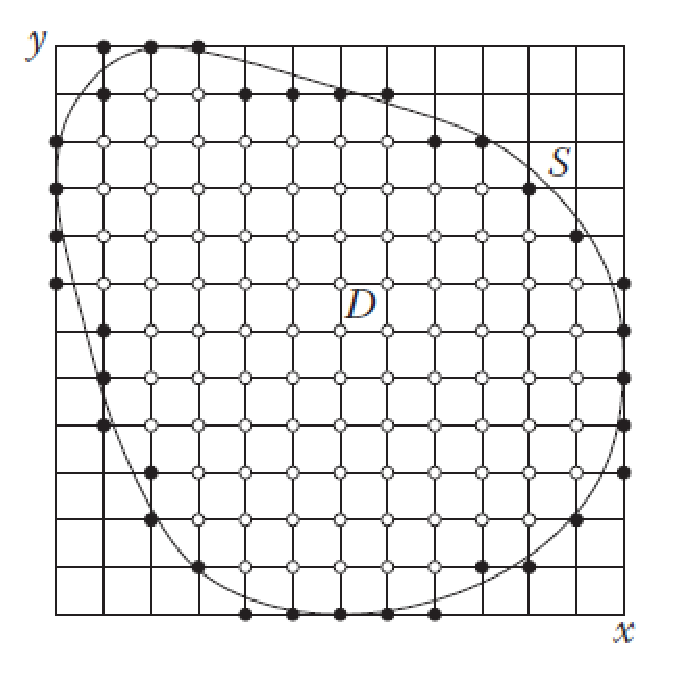
\includegraphics[scale=0.5]{Imagenes/condicionesEDP_01.eps}
	\caption{Malla/rejilla para implementar la solución. Los puntos negros indican los valores de frontera, mientras que los puntos blancos, es donde debe de calcularse la solución.}
\end{figure}
\end{frame}
\begin{frame}
\captionsetup{font=scriptsize,labelfont=scriptsize}
\frametitle{Condiciones con valores iniciales}
\begin{figure}
	\centering
	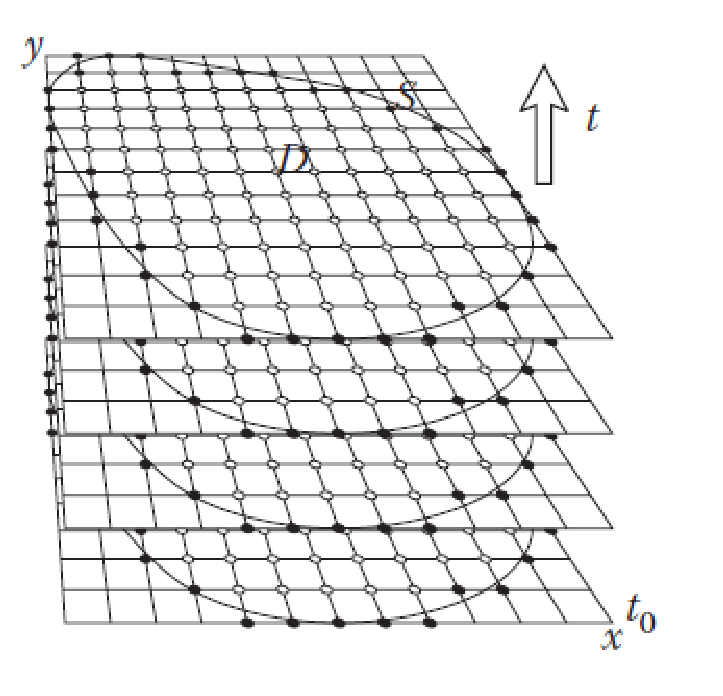
\includegraphics[scale=0.45]{Imagenes/condicionesEDP_02.eps}
	\caption{Se parte de un tiempo inicial $t_{0}$ y evoluciona en el tiempo $t$. Los puntos negros indican los valores de frontera, mientras que los puntos blancos, es donde debe de calcularse la solución.}
\end{figure}
\end{frame}
\begin{frame}
\frametitle{Solución a los problemas}
Aunque el objetivo principal de ambos tipos de problemas es el cálculo de la solución en una red espacial, la solución de estado estacionario para problemas con CDF se determina mediante un proceso numérico que converge simultáneamente en todo el dominio $D$.
\end{frame}
\begin{frame}
\frametitle{Solución a los problemas}
Mientras que en el caso de valores iniciales, la solución de todos los puntos en el dominio espacial, se propagan de manera recursiva en el tiempo, iniciando la solución a partir del instante $t_{0}$.
\end{frame}
\section{Solución de EDP Elípticas}
\frame{\tableofcontents[currentsection, hideothersubsections]}
\subsection{CDF para EDP Elípticas}
\begin{frame}
\frametitle{Problemas CDF para EDP Elípticas}
Para revisar el proceso de discretización para problemas de CDF, consideremos la ecuación 2D de la ecuación de Poisson:
\begin{equation}
\nabla^{2} \: u(x, y) = \dfrac{\partial^{2} u}{\partial x^{2}} + \dfrac{\partial^{2} u}{\partial y^{2}} = f(x, y)
\label{eq:ecuacion_13_01}
\end{equation}
\end{frame}
\begin{frame}
\frametitle{Problemas CDF para EDP Elípticas}
Escogemos un dominio rectangular de integración 
\[ D = [x_{\mbox{min}}, x_{\mbox{max}} ] \times [y_{\mbox{min}}, y_{\mbox{max}} ]  \]
y se establecen las condiciones de frontera mixtas
\begin{equation}
\left[ \alpha \: u + \beta \: \dfrac{\partial u}{\partial n} \right]_{(x, y) \in S} = \gamma
\label{eq:ecuacion_13_02}
\end{equation}
donde $\alpha(x, y)$, $\beta(x, y)$ y $\gamma(x, y)$ son funciones definidas en el dominio $S$.
\end{frame}
\begin{frame}
\frametitle{Problemas CDF para EDP Elípticas}
En particular, tenemos
\setbeamercolor{item projected}{bg=red!70!black,fg=white}
\setbeamertemplate{enumerate items}{%
\usebeamercolor[bg]{item projected}%
\raisebox{1.5pt}{\colorbox{bg}{\color{fg}\footnotesize\insertenumlabel}}%
}
\begin{enumerate}[<+->]
\item \emph{condiciones de Dirichlet} para $\beta = 0$ (valores de solución fijos)
\item \emph{condiciones de Neumann} para $\alpha = 0$ (derivadas normales fijas)
\item \emph{condiciones uniformes} para $\gamma = 0$
\end{enumerate}
\end{frame}
\begin{frame}
\frametitle{Uso de diferencias finitas}
Siguiendo la aproximación por el método de diferencias finitas, acotamos la solución para los valores $N_{x} \times N_{y}$ tal que $u_{ij} = u(x_{i}, y_{j})$ en los nodos de la malla espacial definida por
\begin{align*}
x_{i} = x_{\text{min}} + (i - 1) \: h_{x}, \hspace{0.5cm} i = 1, 2, \ldots, N_{x} \\
y_{i} = y_{\text{min}} + (j - 1) \: h_{y}, \hspace{0.5cm} j = 1, 2, \ldots, N_{y}
\end{align*}
\\
\bigskip
\pause
donde $h_{x}$ y $h_{y}$ corresponde al espaciamiento en la malla en las dos direcciones.
\end{frame}
\begin{frame}
\frametitle{Malla para la solución}
\captionsetup{font=small,labelfont=small}
\begin{figure}
	\centering
	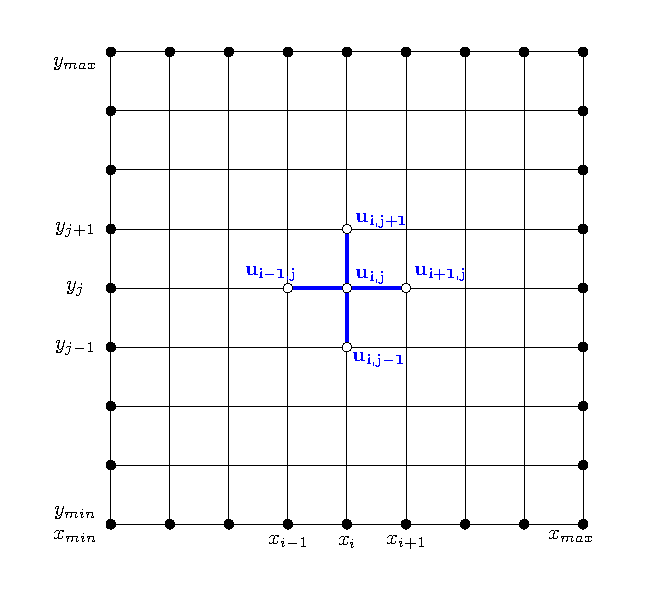
\includegraphics[scale=0.6]{Imagenes/mallaSolucionEDP_01.eps}
	\caption{Discretización de la malla para resolver la EDP.}
	\label{fig:figura_01}
\end{figure}
\end{frame}
\begin{frame}
\frametitle{Uso de diferencias finitas}
Similarmente a las técnicas de diferencias finitas, nos aproximamos al operador laplaciano $\nabla^{2}$ partiendo de la serie de Taylor de la solución en los puntos interiores del dominio $D$.
\\
\bigskip
En particular, a lo largo de la dirección $x$ tenemos, respectivamente, las diferencias hacia atrás y hacia delante:
\end{frame}
\begin{frame}
\frametitle{Uso de diferencias finitas}
Diferencias hacia atrás y hacia adelante
\fontsize{12}{12}\selectfont
\begin{align*}
u_{i-1, j} &= u_{i, j} - \dfrac{h_{x}}{1!} \left( \dfrac{\partial u}{\partial x} \right)_{i, j} + \dfrac{h_{x}^{2}}{2!} \left( \dfrac{\partial^{2} u}{\partial x^{2}} \right)_{i, j} - \dfrac{h_{x}^{3}}{3!} \left( \dfrac{\partial^{3} u}{\partial x^{3}} \right)_{i, j} + O(h_{x}^{4})  \\
u_{i+1, j} &= u_{i, j} + \dfrac{h_{x}}{1!} \left( \dfrac{\partial u}{\partial x} \right)_{i, j} + \dfrac{h_{x}^{2}}{2!} \left( \dfrac{\partial^{2} u}{\partial x^{2}} \right)_{i, j} + \dfrac{h_{x}^{3}}{3!} \left( \dfrac{\partial^{3} u}{\partial x^{3}} \right)_{i, j} + O(h_{x}^{4})
\end{align*}
\end{frame}
\begin{frame}
\frametitle{Uso de diferencias finitas}
La expresión de diferencias finitas para la segunda derivada es
\begin{equation}
\left( \dfrac{\partial^{2} u}{\partial x^{2}} \right)_{i,j} = \dfrac{u_{i+1, j} - 2 \: u_{i, j} + u_{i-1,j}}{h_{x}^{2}} + O(h_{x}^{2})
\label{eq:ecuacion_13_03}
\end{equation}
\pause
De manera análoga, para la segunda derivada en la dirección $y$ es:
\begin{equation}
\left( \dfrac{\partial^{2} u}{\partial y^{2}} \right)_{i,j} = \dfrac{u_{i, j+1} - 2 \: u_{i, j} + u_{i, j-1}}{h_{y}^{2}} + O(h_{y}^{2})
\label{eq:ecuacion_13_04}
\end{equation}
\end{frame}
\begin{frame}
\frametitle{Uso de diferencias finitas}
Entonces, para el laplaciano de la función $u$ en el nodo $(x_{i}, y_{i})$, hay un esquema de diferencia en cinco puntos, que se correlaciona con la representación gráfica en la figura (\ref{fig:figura_01})
\end{frame}
\begin{frame}
\frametitle{El laplaciano de $u$}
\begin{align}
\begin{aligned}
\nabla^{2} u(x,y) \vert_{i,j} &= \dfrac{1}{h_{y}^{2}} \: u_{i, j-1} + \dfrac{1}{h_{x}^{2}} \: u_{i-1, j} + \\
&- 2 \: \left( \dfrac{1}{h_{x}^{2}} + \dfrac{1}{h_{y}^{2}} \right) \: u_{i, j}  + \dfrac{1}{h_{x}^{2}} \: u_{i+1, j}  + \\
&+ \dfrac{1}{h_{y}^{2}} \: u_{i, j+1} + O(h_{x}^{2} + h_{y}^{2})
\end{aligned}
\label{eq:ecuacion_13_05}
\end{align}
\end{frame}
\begin{frame}
\frametitle{Uso de diferencias finitas}
Con ello se obtiene la siguiente expresión de diferencias finitas de la ecuación de Poisson en los puntos interiores del dominio $D$:
\begin{align}
\begin{aligned}
\dfrac{1}{h_{y}^{2}} \: u_{i, j-1} &+ \dfrac{1}{h_{x}^{2}} \: u_{i-1, j} - 2 \: \left( \dfrac{1}{h_{x}^{2}} + \dfrac{1}{h_{y}^{2}} \right) \: u_{i, j} + \\
&+ \dfrac{1}{h_{x}^{2}} \: u_{i+1, j} + \dfrac{1}{h_{y}^{2}} \: u_{i, j+1} = f_{i, j} \\
\\
i &= 2, \ldots, N_{x-1}, \hspace{0.7cm} j = 2, \ldots, N_{y-1}
\end{aligned}
\label{eq:ecuacion_13_06}
\end{align}
donde $f_{i, j} = f(x_{i}, y_{j})$.
\end{frame}
\begin{frame}
\frametitle{Discretización del problema}
El sistema lineal (\ref{eq:ecuacion_13_06}), teniendo como incógnitas los valores de la solución $u_{i, j}$ en los nodos de la malla, no contiene realmente suficientes ecuaciones para que la solución sea completamente determinada. 
\end{frame}
\begin{frame}
\frametitle{Discretización del problema}
Por otra parte, el esquema de discretización de cinco puntos empleado para el laplaciano impide la incorporación directa de las condiciones de frontera, que han de ser tratadas por separado.
\end{frame}
\begin{frame}
\frametitle{Discretización del problema}
Muy a menudo, el proceso de discretización de las condiciones de frontera es más intrincado que la discretización de las EDP mismas.
\\
\bigskip
En aras de la claridad, utilizamos en lo siguiente las aproximaciones de orden inferior para las condiciones de frontera mixtas.
\end{frame}
\begin{frame}
\frametitle{Discretización del problema}
Concretamente, considerando que las derivadas normales son positivas si están orientadas hacia fuera desde el dominio $D$, las condiciones límite a la izquierda y a la derecha ($i = 1$ e $i = N_{x}$) pueden expresarse como:
\[ \alpha_{j}^{x_{\text{\tiny{min}}}} \: u_{1, j} + \beta_{j}^{x_{\text{\tiny{min}}}} \: \dfrac{u_{1, j} - u_{2, j}}{h_{x}} = \gamma_{j}^{x_{\text{\tiny{min}}}} \hspace{1cm} i = 1  \]
\[ \alpha_{j}^{x_{\mbox{\tiny{max}}}} \: u_{N_{x}, j} + \beta_{j}^{x_{\text{\tiny{max}}}} \: \dfrac{u_{N_{x}, j} - u_{N_{x-1}, j}}{h_{x}} = \gamma_{j}^{x_{\text{\tiny{max}}}} \hspace{1cm} i = N_{x} \]
\[ j = 1, \ldots, N_{y}  \]
\end{frame}
\begin{frame}
\frametitle{Discretización del problema}
De manera similar, las condiciones de discretización para la frontera inferior y superior ($j = 1$ y $N_{y}$)
\[ \alpha_{i}^{y_{\text{\tiny{min}}}} \: u_{i, 1} + \beta_{i}^{y_{\text{\tiny{min}}}} \: \dfrac{u_{i, 1} - u_{i, 2}}{h_{y}} = \gamma_{i}^{x_{\text{\tiny{min}}}} \hspace{1cm} j = 1  \]
\[ \alpha_{i}^{y_{\text{\tiny{max}}}} \: u_{i, N} + \beta_{i}^{y_{\text{\tiny{max}}}} \: \dfrac{u_{i, N_{y}} - u_{i, N_{y-1}}}{h_{y}} = \gamma_{i}^{y_{\text{\tiny{max}}}} \hspace{1cm} j = N_{y} \]
\[ i = 1, \ldots, N_{x}  \]
\end{frame}
\begin{frame}
\frametitle{Simplificación en la notación}
Para simplificar las ecuaciones discretizadas y las CDF, definimos las siguientes cantidades
\begin{equation}
k_{x} = \dfrac{1}{h_{x}^{2}}, \hspace{0.5cm} k_{y} = \dfrac{1}{h_{y}^{2}}, \hspace{0.5cm} k_{xy} = 2 \: \left( \dfrac{1}{h_{x}^{2}} + \dfrac{1}{h_{y}^{2}} \right)
\label{eq:ecuacion_13_07}
\end{equation}
\end{frame}
\begin{frame}
\frametitle{Simplificación de las CDF}
Los coeficientes de frontera quedan:
\begin{equation}
\begin{aligned}
\bar{\beta}_{i}^{y {\text{\tiny{min}}}} &= \beta_{i}^{y {\text{\tiny{min}}}} / \left( \alpha_{i}^{y {\text{\tiny{min}}}} \: h_{y}  + \beta_{i}^{y{\mbox{\tiny{min}}}} \right), \\
\bar{\beta}_{i}^{y {\text{\tiny{max}}}} &= \beta_{i}^{y {\text{\tiny{max}}}} / \left( \alpha_{i}^{y {\text{\tiny{max}}}} \: h_{y}  + \beta_{i}^{y{\mbox{\tiny{max}}}} \right), \\
\bar{\beta}_{j}^{x {\text{\tiny{min}}}} &= \beta_{x}^{x {\text{\tiny{min}}}} / \left( \alpha_{j}^{x {\text{\tiny{min}}}} \: h_{x}  + \beta_{j}^{x {\mbox{\tiny{min}}}} \right), \\
\bar{\beta}_{j}^{x {\text{\tiny{max}}}} &= \beta_{j}^{x {\text{\tiny{max}}}} / \left( \alpha_{j}^{x {\text{\tiny{max}}}} \: h_{x}  + \beta_{j}^{x {\mbox{\tiny{max}}}} \right)
\end{aligned}
\label{eq:ecuacion_13_08a}
\end{equation}
\end{frame}
\begin{frame}
\frametitle{Simplificación de las CDF}
Los coeficientes de frontera quedan:
\begin{equation}
\begin{aligned}
\bar{\gamma}_{i}^{y {\text{\tiny{min}}}} &= \gamma_{i}^{y {\text{\tiny{min}}}} / \left( \alpha_{i}^{y {\text{\tiny{min}}}} + \beta_{i}^{y{\text{\tiny{min}}}} / h_{y} \right), \\
\bar{\gamma}_{i}^{y {\text{\tiny{max}}}} &= \gamma_{i}^{y {\text{\tiny{max}}}} / \left( \alpha_{i}^{y {\text{\tiny{max}}}} + \beta_{i}^{y{\text{\tiny{max}}}} / h_{y} \right), \\
\bar{\gamma}_{j}^{x {\text{\tiny{min}}}} &= \gamma_{j}^{x {\text{\tiny{min}}}} / \left( \alpha_{j}^{x {\text{\tiny{min}}}} + \beta_{j}^{x {\text{\tiny{min}}}} / h_{x} \right), \\
\bar{\gamma}_{j}^{x {\text{\tiny{max}}}} &= \gamma_{j}^{x {\text{\tiny{max}}}} / \left( \alpha_{j}^{x {\text{\tiny{max}}}} + \beta_{j}^{x {\text{\tiny{max}}}} / h_{x} \right)
\end{aligned}
\label{eq:ecuacion_13_08b}
\end{equation}
\end{frame}
\begin{frame}
\frametitle{Sistema completo discretizado}
Con esto, el sistema lineal completo resultante de la discretización de la ecuación de Poisson y las condiciones de frontera mixtas adjuntas toma la siguiente forma:
\end{frame}
\begin{frame}
\frametitle{Sistema completo 1/3}
Para la frontera inferior
\begin{equation}
u_{i, 1} - \bar{\beta}_{i}^{y {\text{\tiny{min}}}} \: u_{i, 2} = \bar{\gamma}_{i}^{y {\text{\tiny{min}}}}, \hspace{0.5cm} i = 1, \ldots, N_{x}, \hspace{0.3cm} j = 1
\label{eq:ecuacion_13_09}
\end{equation}
\pause
Para la frontera izquierda
\begin{equation}
u_{i, j} - \bar{\beta}_{i}^{y {\text{\tiny{min}}}} \: u_{2, j} = \bar{\gamma}_{i}^{y {\text{\tiny{min}}}}, \hspace{0.5cm} i = 1, \hspace{0.3cm} j = 2, \ldots, N_{y} - 1
\label{eq:ecuacion_13_10}
\end{equation}
\end{frame}
\begin{frame}
\frametitle{Sistema completo 2/3}
Para los puntos interiores
\begin{equation}
\begin{aligned}
k_{y} \: u_{i, j-1} &+ k_{x} \: u_{i-1, j} - k_{xy} \: u_{i, j} + k_{x} \: u_{i+1, j} + \\
&+ k_{y} \: u_{i, j+1} =  f_{i,j} \\
i &= 2, \ldots, N_{x} - 1, \hspace{1cm} j = 2, \ldots, N_{y} - 1 \hspace{2cm}
\end{aligned}
\label{eq:ecuacion_13_11}
\end{equation}
\end{frame}
\begin{frame}
\frametitle{Sistema completo 3/3}
Para la frontera derecha
\begin{equation}
- \bar{\beta}_{j}^{x {\text{\tiny{max}}}} \:  u^{}_{N_{x-1}, j} + u^{}_{N_{x},j}  =  \bar{\gamma}_{j}^{x {\text{\tiny{max}}}} \hspace{0.5cm} i = N_{x}, \hspace{0.3cm} j = 2, \ldots, N_{y} - 1
\label{eq:ecuacion_13_12}
\end{equation}
\pause
Para la frontera superior
\begin{equation}
- \bar{\beta}_{j}^{y {\text{\tiny{max}}}} \:  u^{}_{i, N_{y-1}} + u^{}_{i, N_{y}}  =  \bar{\gamma}_{i}^{y {\text{\tiny{max}}}} \hspace{0.5cm} i = 1, \ldots, N_{x}, \hspace{0.3cm} j = N_{y}
\label{eq:ecuacion_13_13}
\end{equation}
\end{frame}
\begin{frame}
\frametitle{Re-escribiendo el sistema}
El sistema discretizado completo se puede re-escribir de una forma general, lo que ayuda a revelar su estructura:
\begin{equation}
\begin{aligned}
a_{i}^{j} \: u_{i, j-1} &+ b_{ai}^{j} \: u_{i-1, j} + b_{bi}^{j} \: u_{i, j} + \\
&+ b_{ci}^{j} \: u_{i+1, j} + c_{i}^{j} \: u_{i, j+1} = d_{i}^{j} \\
&i = 1, \ldots, N_{x}, \hspace{0.5cm} j = 1, \ldots, N_{y}
\end{aligned}
\label{eq:ecuacion_13_14}
\end{equation}
\end{frame}
\begin{frame}
\frametitle{Re-escribiendo el sistema}
Teniendo en cuenta que la ecuación discretizada centrada alrededor del nodo malla $(i, j)$ no solo conecta los cinco valores vecinos $(u_{i, j-1}, u_{i-1, j}, u_{i,j}, u_{i+1, j}, u_{i, j+1})$, sino todos los valores en los tres renglones contiguos $j-1, j, j+1$.
\end{frame}
\begin{frame}
\frametitle{Re-escribiendo el sistema}
 El sistema puede expresarse como
\begin{equation}
\begin{aligned}
\sum_{i^{\prime} = 1}^{N_{x}} &\left[ A_{ii^{\prime}}^{j} \: u_{i^{\prime}, j-1} + B_{ii^{\prime}}^{j} \: u_{i^{\prime}, j} + C_{ii^{\prime}}^{j} \: u_{i^{\prime}, j+1}  \right] = d_{i}^{j} \\
&i = 1, \ldots, N_{x} \hspace{0.5cm} j = 1, \ldots, N_{y}
\end{aligned}
\label{eq:ecuacion_13_15}
\end{equation}
\end{frame}
\begin{frame}
\frametitle{Re-escribiendo el sistema}
Donde los bloques $N_{x} \times N_{x}$ de
\begin{align*}
\mathbf{A}^{j} &= [A_{ii^{\prime}}^{j}]_{N_{x} N_{x}} \\
\mathbf{B}^{j} &= [B_{ii^{\prime}}^{j}]_{N_{x} N_{x}} \\
\mathbf{C}^{j} &= [C_{ii^{\prime}}^{j}]_{N_{x} N_{x}} \\
\end{align*}   
tienen los siguientes elementos:
\end{frame}
\begin{frame}
\frametitle{Re-escribiendo el sistema}
\begin{equation}
\begin{aligned}
A_{ii^{\prime}}^{j} &= a_{i}^{j} \: \delta_{ii^{\prime}} \\
B_{ii^{\prime}}^{j} &= \begin{cases}
b_{ai}^{j} & \mbox{ si } i^{\prime} = i-1 \\
b_{bi}^{j} & \mbox{ si } i^{\prime} = i \\
b_{ci}^{j} & \mbox{ si } i^{\prime} = i+1 \\
0 & \mbox{ si } i^{\prime} \neq i, i \pm 1 \end{cases} \\
C_{ii^{\prime}}^{j} &= c_{i}^{j} \: \delta_{ii^{\prime}}
\end{aligned}
\label{eq:ecuacion:13_16}
\end{equation}
\end{frame}
\begin{frame}
\frametitle{Sistema matricial en banda}
Usando estos bloques, del sistema matricial completo se puede ver que forma un bloque trigiadonal y su estructura en banda es la siguiente:
\end{frame}
{\setbeamercolor{background canvas}{bg=white}
\begin{frame}
\frametitle{Sistema tridiagonal y en banda}
\begin{figure}
	\centering
	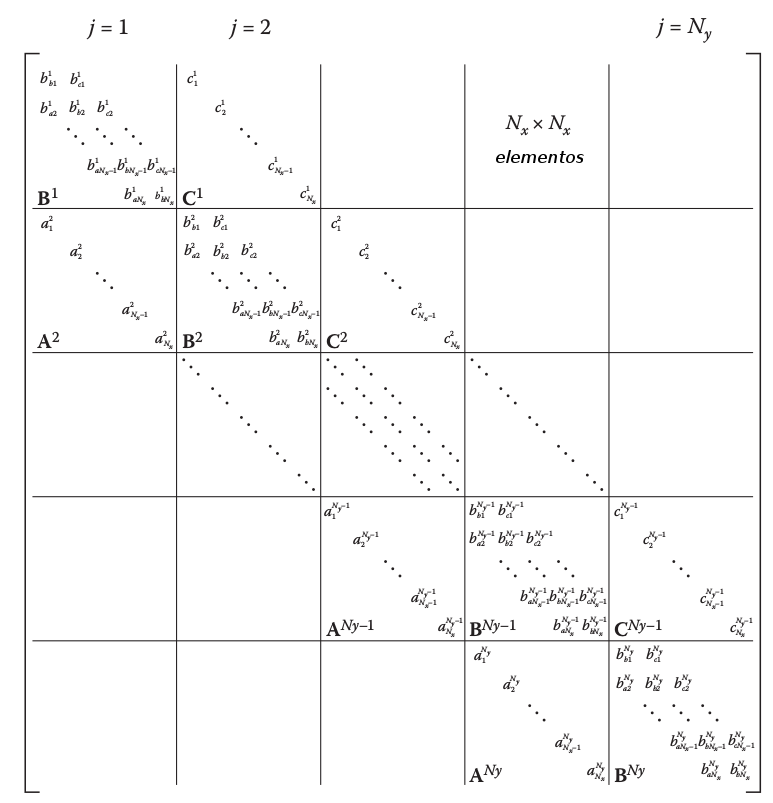
\includegraphics[scale=0.27]{Imagenes/Sistema_Matricial_Completo.png}
\end{figure}    
\end{frame}
}
\begin{frame}
\frametitle{Ajustado el sistema discretizado}
Al definir los vectores $\mathbf{u}^{j} = [u_{i^{\prime}, j}]_{N_{x}}$ y $\mathbf{d}^{j} = [d_{i}^{j}]_{N_{x}}$, con $\mathbf{u}^{j}$ teniendo como componentes los valores de solución $N_{x}$ en la fila $j$ y $\mathbf{d}^{j}$ que contienen los términos correspondientes del lado derecho, el sistema discretizado toma la forma:
\begin{equation}
\mathbf{A}^{j} \: \mathbf{u}^{j-1} + \mathbf{B}^{j} \: \mathbf{u}^{j+1} +  \mathbf{C}^{j} \: \mathbf{u}^{j+1} = \mathbf{d}^{j}, \hspace{0.5cm} j = 1, 2, \ldots, N_{y}
\label{eq:ecuacion_13_17}
\end{equation}
\end{frame}
\begin{frame}
\frametitle{Ajustando el sistema discretizado}
Vemos un conjunto de ecuaciones matriciales conectando los vectores $\mathbf{u}^{j-1}$, $\mathbf{u}^{j}$ y $\mathbf{u}^{j+1}$, que son, las soluciones de los renglones $j-1$, $j$ y $j+1$, respectivamente.
\end{frame}
\begin{frame}
\frametitle{Ajustando el sistema discretizado}
En notación matricial, la estructura en bloques tridiagonal puede leerse como:
\pause
\fontsize{12}{12}\selectfont
\begin{equation}
\begin{bmatrix}
\mathbf{B^{1}} & \mathbf{C^{1}} & & & \\
\mathbf{A^{2}} & \mathbf{B^{2}} & \mathbf{C^{2}} & & \\
 & \ddots & \ddots & \ddots & \\
 & & \mathbf{A^{N_{y}}-1} & \mathbf{B^{N_{y}}-1} & \mathbf{C^{N_{y}}-1}& \\
 & & & \mathbf{A}^{N_{y}} & \mathbf{B}^{N_{y}} 
\end{bmatrix}
\begin{bmatrix}
\mathbf{u}^{1} \\
\mathbf{u}^{2} \\
\vdots \\
\mathbf{u}^{N_{y} - 1} \\
\mathbf{u}^{N_{y}}
\end{bmatrix} = 
\begin{bmatrix}
\mathbf{d}^{1} \\
\mathbf{d}^{2} \\
\vdots \\
\mathbf{d}^{N_{y} - 1} \\
\mathbf{d}^{N_{y}}
\end{bmatrix}
\label{eq:ecuacion_13_18}
\end{equation}
\end{frame}
\begin{frame}
\frametitle{Solución del sistema completo}
El sistema (\ref{eq:ecuacion_13_18}) puede resolverse, en principio, usando los dos tipos de métodos que consideran la estructura escasa de la matriz:
\setbeamercolor{item projected}{bg=red!70!black,fg=white}
\setbeamertemplate{enumerate items}{%
\usebeamercolor[bg]{item projected}%
\raisebox{1.5pt}{\colorbox{bg}{\color{fg}\footnotesize\insertenumlabel}}%
}
\begin{enumerate}[<+->]
\item \emph{Métodos directos: } que utilizan la inversión recursiva de los bloques que componen a la matriz.
\item \emph{Métodos indirectos: } como el de Jacobi o Gauss-Seidel y de sobrerrelajación.
\end{enumerate}
\end{frame}
\begin{frame}
\frametitle{Estrategia de solución}
Debido a la implementación menos elaborada y al escalamiento más favorable de los cálculos con el tamaño del sistema, para problemas con más de dos dimensiones o con límites de dominio complejos, los métodos iterativos resultan ser preferibles para resolver el sistema lineal obtenido al discretizar la EDP con CDF.
\end{frame}
\begin{frame}
\frametitle{Estrategia de solución}
Por lo tanto, limitamos la siguiente discusión al método iterativo de \emph{Gauss-Seidel}, que muestra en la práctica un espectro más amplio de aplicaciones, que también es adecuado para resolver problemas de valores propios para EDP.
\end{frame}
\begin{frame}
\frametitle{Solución}
Podemos re-escribir el sistema con la siguiente forma general
\begin{equation}
\mathbf{A \cdot u} =  \mathbf{d}
\label{eq:ecuacion_13_19} 
\end{equation}
\pause
Y considerar la descomposición:
\begin{equation}
\mathbf{A} = \mathbf{L} + \mathbf{D} + \mathbf{U}
\label{eq:ecuacion_13_20}
\end{equation}
donde: $\mathbf{L}$ es una matriz triangular inferior, $\mathbf{D}$ es una matriz diagonal, $\mathbf{U}$ es una matriz triangular superior.
\end{frame}
\begin{frame}
\frametitle{Solución}
En el \emph{Método de Jacobi}, los elementos de la diagonal se expresan y la solución se itera de acuerdo a la relación:
\begin{align*}
\mathbf{D} \cdot \mathbf{u}^{(r)} = \mathbf{d} - (\mathbf{L} + \mathbf{U}) \cdot \mathbf{u}^{(r-1)}
\end{align*}
o equivalentemente
\begin{equation}
\mathbf{u}^{(r)} = \mathbf{D}^{-1} \cdot \left[ \mathbf{d} - (\mathbf{L} + \mathbf{U}) \cdot \mathbf{u}^{(r-1)} \right]
\label{eq:ecuacion_13_21}
\end{equation}
donde $r = 1, 2, \ldots$ es el orden de la aproximación a la solución.
\end{frame}
\begin{frame}
\frametitle{Solución}
Como $\mathbf{D}$ es diagonal, la inversa $\mathbf{D}^{-1}$ también es diagonal y contiene simplemente las inversas de los elementos diagonales de $\mathbf{D}$.
\\
\bigskip
El método de Jacobi converge para las matrices que son diagonalmente dominantes y esta condición generalmente se satisface en el marco de las metodologías de diferencias finitas.
\end{frame}
\begin{frame}
\frametitle{Solución}
Refiriéndose específicamente a la ecuación (\ref{eq:ecuacion_13_11} para los puntos de malla interior de los sistemas discretizados (\ref{eq:ecuacion_13_09}) - (\ref{eq:ecuacion_13_13}), los componentes de solución diagonal son los que están situados en el centro de los esquemas de discretización tipo estrella, es decir, $u_{i,j}$.
\end{frame}
\begin{frame}
\frametitle{Solución}
Correspondientemente, la solución se itera en función de la relación de recurrencia:
\begin{align}
\begin{aligned}
u_{i,j}^{(r)} &= \left[ k_{x} \: \left( u_{i-1,j}^{(r-1)} + u_{i+1, j}^{(r-1)} \right) + \right. \\
&+ \left. k_{y} \: \left( u_{i,j-1}^{(r-1)} + u_{i, j+1}^{(r-1)} \right) - f_{i,j} \right] / k_{xy}
\end{aligned}
\label{eq:ecuacion_13_22} 	
\end{align}
\pause
Está definiendo para el método de Jacobi, que todos los valores de solución empleados en el lado derecho provienen de la iteración anterior: $(r - 1)$.
\end{frame}
\begin{frame}
\frametitle{Solución}
Suponiendo que el algoritmo se ejecuta dentro de los bucles anidados, en orden creciente de los índices $i$ y $j$ al calcular $u_{i,j}^{(r)}$, los componentes actualizados de $u_{i, j-1}^{(r)}$ y $u_{i-1, j}^{(r)}$ ya están disponibles.
\end{frame}
\begin{frame}
\frametitle{Solución}
Su uso inmediato es específico en el método de Gauss-Seidel y la correspondiente relación de recurrencia formal toma la forma:
\begin{align}
\begin{aligned}
u_{i,j}^{(r)} &= \left[ k_{x} \: \left( u_{i-1,j}^{(r)} + u_{i+1, j}^{(r-1)} \right) + \right. \\
&+ \left. k_{y} \: \left( u_{i,j-1}^{(r)} + u_{i, j+1}^{(r-1)} \right) - f_{i,j} \right] / k_{xy}
\end{aligned}
\label{eq:ecuacion_13_23} 	
\end{align}
\end{frame}
\begin{frame}
\frametitle{Solución}
Por lo tanto, a diferencia del método de Jacobi, $u_{i,j}^{(r)}$ es calculado usando los más recientes componentes de $u_{i,j-1}^{(r)}$ y $u_{i-1, j}^{(r)}$, y no de sus predecesores $u_{i,j-1}^{(r-1)}$ y $u_{i-1, j}^{(r-1)}$.
\end{frame}
\begin{frame}
\frametitle{Solución}
Además de la velocidad de convergencia mejorada, el método de Gauss-Seidel también requiere una sola matriz (no dos) para almacenar la solución.
\\
\bigskip
Este arreglo puede contener al mismo tiempo componentes de ambas aproximaciones $\mathbf{u}^{(r-1)}$ y $\mathbf{u}^{(r)}$, que se actualizan continuamente y se pueden utilizar inmediatamente después de su cálculo.
\end{frame}
\begin{frame}
\frametitle{Ecuaciones obtenidas con Gauss-Seidel}
Las ecuaciones que describen la solución iterativa del sistema discretizado (\ref{eq:ecuacion_13_09}) -  (\ref{eq:ecuacion_13_13}) con condiciones de frontera mixtas, basadas en el método de Gauss-Seidel, ahora se pueden compilar de la siguiente manera:
\end{frame}
\begin{frame}
\frametitle{Ecuaciones obtenidas con Gauss-Seidel 1/3}
Para la frontera inferior
\begin{equation}
u_{i, 1}^{(r)} = \bar{\beta}_{i}^{y {\text{\tiny{min}}}} \: u_{1,2}^{(r-1)} + \bar{\gamma}_{i}^{y {\text{\tiny{min}}}}, \hspace{0.5cm} i = 1, \ldots, N_{x}, \hspace{0.3cm} j = 1
\label{eq:ecuacion_13_24}
\end{equation}
\pause
Para la frontera izquierda
\begin{equation}
u_{i, j}^{(r)} = \bar{\beta}_{i}^{x {\text{\tiny{min}}}} \: u_{2, j}^{(r-1)} + \bar{\gamma}_{j}^{x {\text{\tiny{min}}}}, \hspace{0.5cm} i = 1, \hspace{0.3cm} j = 2, \ldots, N_{y} - 1
\label{eq:ecuacion_13_25}
\end{equation}
\end{frame}
\begin{frame}
\frametitle{Ecuaciones obtenidas con Gauss-Seidel 2/3}
Para los puntos interiores
\begin{equation}
\begin{aligned}
u_{i,j}^{(r)} &= \left[ k_{x} \left( u_{i, j-1}^{(r)} u_{i+1, j}^{(r-1)} \right) + \right. \\
&+ \left. k_{y} \left( u_{i, j-1}^{(r)} + u_{i, j+1}^{(r-1)} \right) - f_{i,j} \right] / k_{xy} \\
i &= 2, \ldots, N_{x} - 1, \hspace{1cm} j = 2, \ldots, N_{y} - 1 \hspace{2cm}
\end{aligned}
\label{eq:ecuacion_13_26}
\end{equation}    
\end{frame}
\begin{frame}
\frametitle{Ecuaciones obtenidas con Gauss-Seidel 3/3}
\frametitle{Sistema completo 3/3}
Para la frontera derecha
\begin{equation}
u_{N_{x},j}^{(r)} = \bar{\beta}_{j}^{x {\text{\tiny{max}}}} \:  u_{N_{x-1}, j}^{(r-1)} + \bar{\gamma}_{j}^{x {\text{\tiny{max}}}} \hspace{0.5cm} i = N_{x}, \hspace{0.3cm} j = 2, \ldots, N_{y} - 1
\label{eq:ecuacion_13_27}
\end{equation}
\pause
Para la frontera superior
\begin{equation}
u_{i, N_{y}}^{(r)} = \bar{\beta}_{j}^{y {\text{\tiny{max}}}} \:  u_{N_{x-1}, j}^{(r-1)} + \bar{\gamma}_{i}^{y {\text{\tiny{max}}}} \hspace{0.5cm} i = 1, \ldots, N_{x}, \hspace{0.3cm} j = N_{y}
\label{eq:ecuacion_13_28}
\end{equation}
\end{frame}
\begin{frame}
\frametitle{Punto de paro}
El proceso recursivo (\ref{eq:ecuacion_13_24}) - (\ref{eq:ecuacion_13_28}) continua, en principio, hasta que la \emph{diferencia máxima relativa} entre los componentes de la solución de dos iteraciones consecutivas son menores a una tolerencia definida $\varepsilon$:     
\begin{equation}
\max_{i,j} \vert 1 - u_{ij}^{(r-1)} / u_{ij}^{(r)} \vert \leq \varepsilon
\label{eq:ecuacion_13_29}
\end{equation}
\end{frame}
\begin{frame}
\frametitle{Punto de paro}
Para los componentes que se anulan, este criterio de convergencia debería emplear la diferencia \emph{absoluta} máxima:
\[ \max_{i,j} \vert u_{ij}^{(r)} / u_{ij}^{(r-1)} \vert \]
\end{frame}

\section{Problema de potencial eléctrico}
\frame{\tableofcontents[currentsection, hideothersubsections]}
\subsection{EDP Elíptica: la ecuación de Laplace}

\begin{frame}
\frametitle{Problema de potencial eléctrico}
Nuestro problema es: a partir de una configuración inicial, debemos de calcular el potencial eléctrico para todos los puntos que están dentro de una malla cuadrada.
\end{frame}
\begin{frame}
\frametitle{Problema de potencial eléctrico}
La parte inferior y las orillas de la región están unidos y conectados a \enquote{tierra}, mientras que en la parte superior tenemos un cable conectado a una fuente de voltaje de 100 Volts.
\begin{figure}
	\centering
	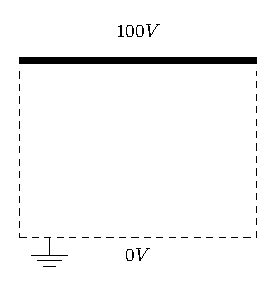
\includegraphics[scale=0.6]{Imagenes/mallaSolucionEDP_02.eps}
\end{figure}
\end{frame}
\begin{frame}
\frametitle{EDP Elíptica, la ecuación de Laplace}
Consideremos que tenemos un cuadrado completo para nuestro problema, de tal manera que los bordes son aislantes y cierran el cuadro.
\end{frame}
\begin{frame}
\frametitle{EDP Elíptica, la ecuación de Laplace}
Dado que conocemos los valores de potencial, tenemos un problema con condiciones de Neumann en la frontera, por lo que la solución es única y estable.
\end{frame}
\begin{frame}
\frametitle{EDP Elíptica, la ecuación de Laplace}
Sabemos de la teoría electrodinámica que el potencial eléctrico $U(x)$ alrededor de una carga estática, satisface la ecuación de Poisson:
\[ \nabla^{2} U(x) = - 4 \pi \rho(x) \]
donde $\rho(x)$ es la densidad de carga.
\end{frame}
\begin{frame}
\frametitle{EDP Elíptica, la ecuación de Laplace}
En las regiones espaciales sin carga, es decir $\rho(x)=0$, el potencial satisface la ecuación de Laplace:
\[ \nabla^{2} U(x) = 0\]
\end{frame}
\begin{frame}
\frametitle{EDP Elíptica, la ecuación de Laplace}
Resolviendo las ecuaciones en 2-D en coordenadas rectangulares:
\[ \dfrac{\partial^{2} U(x,y)}{\partial x^{2}} + \dfrac{\partial^{2} U(x,y)}{\partial y^{2}}  = \left\lbrace \begin{array}{l}
0 \\
- 4\pi \rho(x)
\end{array} \right. \]
\end{frame}
\begin{frame}
\frametitle{Solución del problema}
Para resolver nuestra ecuación 2-D numéricamente, dividimos el espacio en una malla y buscamos la solución para $U$ en cada una de ellas.
\end{frame}
\begin{frame}
\frametitle{Solución del problema}
Como expresaremos derivadas en términos de diferencias finitas de los valores de $U$ para cada elemento de la malla, este es el método de diferencias finitas.
\\
\bigskip
Un método más eficiente pero a la vez más complicado es la técnica del elemento finito que resuelve la EDP para pequeños elementos geométricos.
\end{frame}
\begin{frame}
\frametitle{División de la región de trabajo}
El algoritmo para la ecuación de Laplace: el potencial en un punto $(x,y) = (i,j)$ $\Delta$ es igual al promedio de los valores de potencial de los cuatro puntos vecinos, los nodos con los centros en blanco, corresponden a los valores de potencial constante sobre la frontera.
\end{frame}
{\setbeamercolor{background canvas}{bg=white}
\begin{frame}[plain]
\begin{figure}
	\centering
	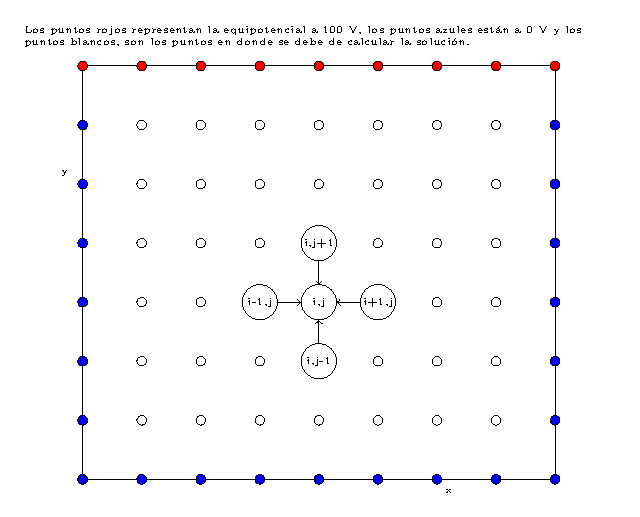
\includegraphics[scale=0.6]{Imagenes/mallaSolucionEDP_03.eps}
\end{figure}
\end{frame}
}
\begin{frame}
\frametitle{Solución del problema}
Usaremos el algoritmo de diferenciación hacia adelante. Sumamos las dos series de Taylor para el potencial: a la derecha e izquierda de $(x,y)$ así como para arriba y abajo de $(x,y)$:
\fontsize{12}{12}\selectfont
\begin{align*}
U(x + \Delta x,y) &= U(x, y) + \dfrac{\partial U}{\partial x} \: \Delta x + \dfrac{1}{2} \dfrac{\partial^{2} U}{\partial x^{2}} \: (\Delta x)^{2} + \ldots \\
U(x - \Delta x,y) &= U(x,y) - \dfrac{\partial U}{\partial x} \: \Delta x + \dfrac{1}{2} \dfrac{\partial^{2} U}{\partial x^{2}} \: (\Delta x)^{2} - \ldots \\
\end{align*}
\end{frame}
\begin{frame}
\frametitle{Solución del problema}
Todos los términos impares se cancelan, al sumar las ecuaciones obtendremos una aproximación por diferencias centrales para las segunda derivada parcial:
\fontsize{12}{12}\selectfont
\begin{align*}
\dfrac{\partial^{2} U(x,y)}{\partial x^{2}} &\simeq \dfrac{U(x+\Delta x, y) + U(x-\Delta x,y)-2 \: U(x,y)}{(\Delta x)^{2}} \\
\dfrac{\partial^{2} U(x,y)}{\partial y^{2}} &\simeq \dfrac{U(x, y+\Delta y) + U(x,y-\Delta y)-2 \: U(x,y)}{(\Delta y)^{2}}
\end{align*}
\end{frame}
\begin{frame}
\frametitle{Solución del problema}
Al sustituir las dos ecuaciones en la ecuación de Laplace, obtenemos una expresión en diferencias finitas para la EDP:
\fontsize{12}{12}\selectfont
\begin{align*}
\dfrac{U(x+\Delta x,y) + U(x-\Delta x, y) - 2 \: U(x,y)}{(\Delta x^{2})} + {} \\
{} + \dfrac{U(x,y+\Delta y) + U(x,y-\Delta y) - 2 \: U(x,y)}{(\Delta y)^{2}} \simeq 0
\end{align*}
\end{frame}
\begin{frame}
\frametitle{Solución del problema}
Asumimos que los puntos en la malla $(x,y)$ tienen el mismo espaciamiento $\Delta x =  \Delta y = \Delta$, por el que el algoritmo toma la sencilla forma:
\begin{align*}
U(x + \Delta, y) + U(x-\Delta, y) + {} \\
U(x,y +\Delta)  + U(x,y - \Delta) - 4 \: U(x,y)= 0
\end{align*}
\end{frame}
\begin{frame}
\frametitle{Solución del problema}
La ecuación muestra una relación entre las soluciones en los cinco puntos.
\\
\bigskip
Cuando $U(x,y)$ se evalúa para $N_{x}$ valores en la malla y para $N_{y}$ valores, obtenemos un conjunto de $N_{x} \times N_{y}$ ecuaciones algebraicas lineales.
\end{frame}
\begin{frame}
Hacemos una aproximación para $U(x,y)$
\begin{eqnarray*}
U(x,y) \simeq	\dfrac{1}{4} \left[ U(x+\Delta ,y) + U(x-\Delta,y) + \right. \\
\left. + U(x,y+\Delta) + U(x,y-\Delta) \right]
\end{eqnarray*}
En términos de posiciones discretas de la malla, las variables $x$, $y$ son:
\[ x = x_{0} + i \Delta, \hspace{1cm} y = y_{0}+ j \Delta, \hspace{0.8cm} i,j = 0,1,\ldots,N_{max-1} \]
\end{frame}
\begin{frame}
\frametitle{Solución del problema}
El algoritmo de diferencias finitas resulta ser:
\[ U_{i,j} = \dfrac{1}{4} [U_{i+1,j} + U_{i-1,j} + U_{i,j+1} + U_{i,j-1}] \]
\begin{figure}
	\centering
	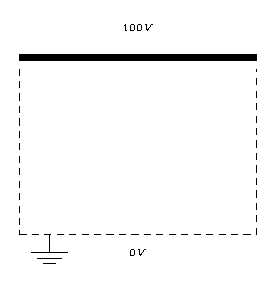
\includegraphics[scale=0.6]{Imagenes/mallaSolucionEDP_04.eps}
\end{figure}
\end{frame}
\subsection{Solución con \python}
\begin{frame}
\frametitle{Implementando el código}
El código tiene cuatro secciones:
\setbeamercolor{item projected}{bg=bananayellow,fg=black}
\setbeamertemplate{enumerate items}{%
\usebeamercolor[bg]{item projected}%
\raisebox{1.5pt}{\colorbox{bg}{\color{fg}\footnotesize\insertenumlabel}}%
}
\begin{enumerate}[<+->]
\item Inicializar todos los puntos de la malla en un potencial de 0 V.
\item Asignar el valor de 100 V a uno de los extremos que corresponden al problema, éste valor debe de permanecer \textbf{constante} durante todo el proceso del algoritmo.
\seti
\end{enumerate}
\end{frame}
\begin{frame}
\frametitle{Implementando el código}
\setbeamercolor{item projected}{bg=bananayellow,fg=black}
\setbeamertemplate{enumerate items}{%
\usebeamercolor[bg]{item projected}%
\raisebox{1.5pt}{\colorbox{bg}{\color{fg}\footnotesize\insertenumlabel}}%
}
\begin{enumerate}[<+->]
\conti
\item El algoritmo se aplica a todos los puntos de la malla (la línea equipotencial de 100 V se mantiene constante)
\item Se grafican los datos con la librería de \funcionazul{matplotlib}.
\end{enumerate}
\end{frame}
{\setbeamercolor{background canvas}{bg=white}
\begin{frame}[fragile]
\frametitle{0. Llamada a las librerías}
\begin{lstlisting}[caption=Llamando a las librerías que se utilizarán, style=FormattedNumber, basicstyle=\linespread{1.1}\ttfamily=\small, columns=fullflexible]
import numpy as np

import matplotlib.pylab as plt

from matplotlib import cm
\end{lstlisting}
\end{frame}
\begin{frame}[fragile]
\frametitle{1. Iniciar la malla}
Se requiere preparar un espacio de trabajo, en este caso, una malla cuadrada de $100$ puntos. Para ello, la construimos mediante un arreglo:
\\
\bigskip
\begin{lstlisting}[caption=Construyendo la malla, style=FormattedNumber, basicstyle=\linespread{1.1}\ttfamily=\small, columns=fullflexible]
Nmax = 100

Niter = 70

V = np.zeros((Nmax, Nmax), float)
\end{lstlisting}
\end{frame}
\begin{frame}[fragile]
\frametitle{2. Asignación de valores iniciales en la malla}
Sin importar la posición de los puntos, les asignamos el valor de cero a todos.
\begin{lstlisting}[basicstyle=\linespread{0.9}\ttfamily\small, columns=fullflexible]
for i in range(100):
    for j in range(100):
        V[i][j] = 0.0
\end{lstlisting}
\end{frame}
\begin{frame}[fragile]
\frametitle{3. Asignación de valores en la frontera}
Corresponde ahora, asignar los valores de la frontera, para los cuales, $V=100$, así pues:
\begin{lstlisting}[caption=Asignando los valores iniciales, style=FormattedNumber, basicstyle=\linespread{1.1}\ttfamily=\small, columns=fullflexible]
for k in range(0, Nmax-1):
    V[k,_0_] = 100.0
\end{lstlisting}
\end{frame}
\begin{frame}[fragile]
\frametitle{4. Algoritmo de iteración}
Una vez determinados los puntos del problema, usamos el siguiente algoritmo de iteración, que se calcula 1000 veces, esto para darle estabilidad a los resultados.
\end{frame}
\begin{frame}[plain, allowframebreaks, fragile]
\frametitle{5. Algoritmo de iteración}
\begin{lstlisting}[caption=Iteración en los puntos, style=FormattedNumber, basicstyle=\linespread{1.1}\ttfamily=\small, columns=fullflexible]
for iter in range(Niter):
    if iter%10 == 0: print(iter)
    for i in range(1, Nmax-2):
        for j in range(1, Nmax-2):
            V[i,j] = 0.25 * (V[i+_1_,j] + V[i-_1_,j] + V[i,j+_1_] + V[i,j-_1_])
\end{lstlisting}
\end{frame}
\begin{frame}[fragile]
\frametitle{6. Graficando los datos obtenidos}
Con el siguiente llamado a librerías gráficas, lo que buscamos es preparar una superficie para representar los datos y ocupar adicionalmente, una barra lateral que nos indica un gradiente tanto de color como de valores, junto con curvas de nivel de los equipotenciales.
\end{frame}
\begin{frame}[plain, allowframebreaks, fragile]
\frametitle{7. Graficando los datos obtenidos}
\begin{lstlisting}[caption=Graficando la solución, style=FormattedNumber, basicstyle=\linespread{1.1}\ttfamily=\small, columns=fullflexible]
x = range(0, Nmax-_1_, 2); y = range(0, 50, 2)

X, Y = plt.meshgrid(x, y)

def functz(V):
    z = V[X, Y]
    return z

Z = functz(V)

fig = plt.figure()

ax = fig.add_\textunderscore_subplot(projection='3d')
surf = ax.plot_\textunderscore_surface(X, Y, Z, rstride=2, cstride=2, linewidth=0.5, cmap=cm.coolwarm)
surf.set_\textunderscore_clim([np.min(Z), np.max(Z)])

ax.set_\textunderscore_zlabel('Voltaje')
ax.set_\textunderscore_xlabel('x')
ax.set_\textunderscore_ylabel('y')

#Para la barra lateral
cbar = fig.colorbar(surf, shrink=0.5, aspect=10)
cbar.ax.set_\textunderscore_ylabel('Potencial electrico', rotation=270)
cset = ax.contourf(X,Y,Z, zdir='z', offset=-50, cmap=cm.coolwarm)

ax.set_\textunderscore_zlim(-50, 100)

plt.show()
\end{lstlisting}
\end{frame}
}
\begin{frame}
\frametitle{8. Graficando los datos obtenidos}
Nótese que aunque importamos matplotlib, es necesario utilizar la librería \funcionazul{cm} que nos ofrece un mapa de colores.
\\
\medskip
Llamamos con la variable \funcionazul{fig} para referirnos posteriormente en el código al espacio de trabajo con la gráfica, la variable \funcionazul{ax}, de igual manera, es una referencia para los elementos en específico del objeto en tres dimensiones.
\end{frame}
{\setbeamercolor{background canvas}{bg=white}
\begin{frame}[fragile]
\frametitle{8. Graficando los datos obtenidos}
\begin{figure}
	\centering
	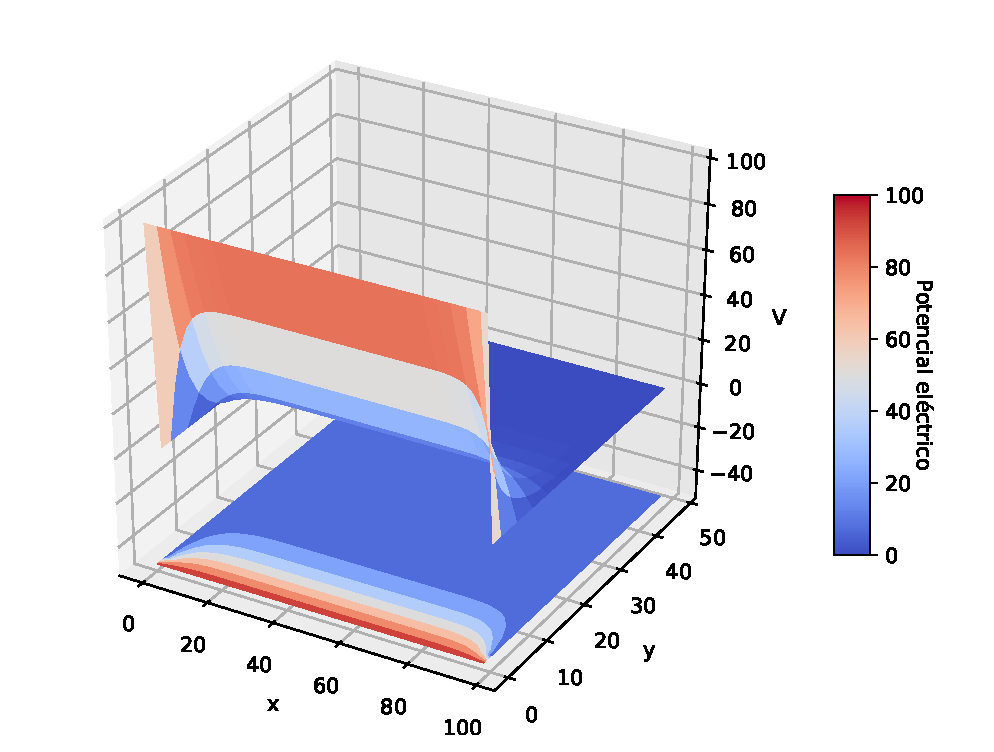
\includegraphics[scale=0.6]{Imagenes/Solucion_Laplace_01.eps} 
\end{figure}
\end{frame}
}
\subsection{Ejercicios a cuenta de examen}
\begin{frame}
\frametitle{1. Problema a cuenta de examen}
Ahora haremos un cambio en la geometría y dificultad del problema: vamos a considerar el caso de un condensador de placas paralelas, tal como se muestra en  la siguiente figura.
\end{frame}
\captionsetup[figure]{labelfont={color=blue}}
\begin{frame}
\frametitle{Geometría para el problema}
\begin{figure}
	\centering
	\includestandalone{Figuras/ejercicio_01_Tarea_Examen}
	\caption{Los valores de $w$ y de $d$ los estableces antes de proponer la solución, recuerda que cada barra mantiene el voltaje durante las iteraciones.}
\end{figure}
\end{frame}
\begin{frame}
\frametitle{Consideraciones}
Tienes que resolver la ecuación para calcular el potencial en cada punto, toma en cuenta lo siguiente:
\setbeamercolor{item projected}{bg=red!70!black,fg=white}
\setbeamertemplate{enumerate items}{%
\usebeamercolor[bg]{item projected}%
\raisebox{1.5pt}{\colorbox{bg}{\color{fg}\footnotesize\insertenumlabel}}%
}
\begin{enumerate}[<+->]
\item Usa un cuadro de $100 \times 100$ para tener una mejor visualización.
\item Las líneas con potencial constante, tienen una longitud $w$, tal que $w<L$  (es decir, no van de un extremo al otro)
\seti
\end{enumerate}
\end{frame}
\begin{frame}
\frametitle{Consideraciones}
\setbeamercolor{item projected}{bg=red!70!black,fg=white}
\setbeamertemplate{enumerate items}{%
\usebeamercolor[bg]{item projected}%
\raisebox{1.5pt}{\colorbox{bg}{\color{fg}\footnotesize\insertenumlabel}}%
}
\begin{enumerate}[<+->]
\conti
\item Hay una separación $d$ que es constante entre las dos líneas de equipotencial.
\item Una vez con la solución de la EDP, grafica tus resultados.
\end{enumerate}
\end{frame}
{\setbeamercolor{background canvas}{bg=white}
\begin{frame}[fragile]
\frametitle{Solución al problema de las placas}
\begin{figure}
	\centering
	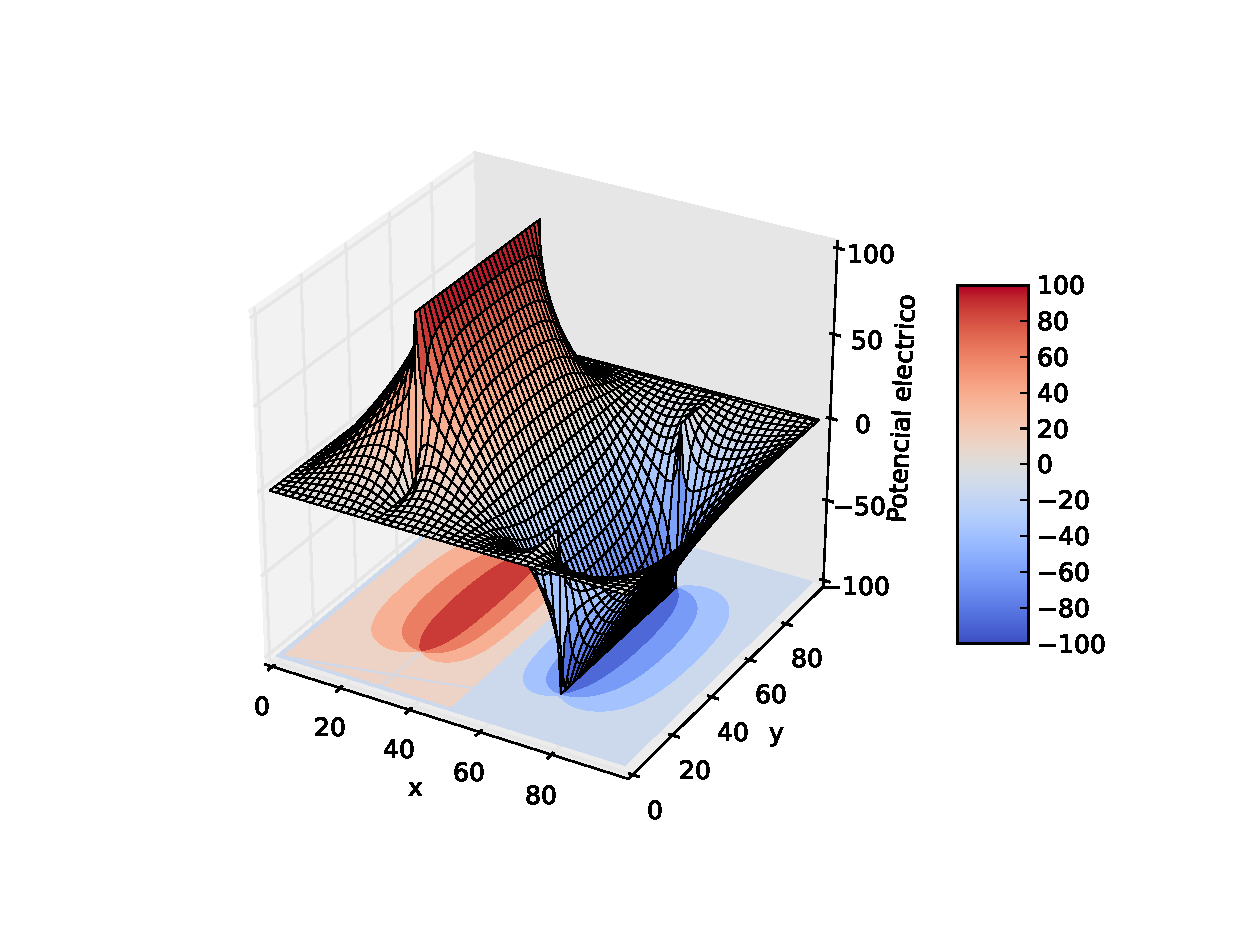
\includegraphics[scale=0.45]{Imagenes/Potencial02.eps} 
\end{figure}
\end{frame}
}
% \begin{frame}
% \frametitle{2. Problema a cuenta del examen}
% Resuelve la ecuación de Laplace con el siguiente arreglo donde la placa cuadrada conductora se encuentra a $1$ volt(geométricamente se localiza en el centro de la placa exterior, por lo que deberás de determinar su tamaño) mientras que la placa cuadrada exterior, se encuentra a $0$ volts.
% \end{frame}
% {\setbeamercolor{background canvas}{bg=white}
% \begin{frame}
% \frametitle{2. Problema a cuenta del examen}
% \begin{figure}
% 	\centering
% 	\includestandalone{Figuras/ejercicio_02_Tarea_Examen}
% 	\caption{Las dimensiones de cada cuadrado las determinas nuevamente antes del iniciar la solución.}
% \end{figure}
% \end{frame}
% }
% \begin{frame}
% \frametitle{3. Problema a cuenta del examen}
% Desarrolla un esquema numérico para resolver la ecuación de Poisson
% \[ \nabla^{2} \phi (r,\theta) = - \rho (r, \theta) / \epsilon_{0} \]
% en coordenadas polares. 
% \\
% \bigskip
% Considera que la geometría en la frontera es un anillo circular con potenciales dados, para el radio interno es $\phi(a,\theta)$, y para el radio externo $\phi(b,\theta)$. Prueba tu solución asignando valores de potencial al problema.
% \end{frame}
%\begin{frame}
%\frametitle{Tips}
%La ecuación de Poisson en coordenadas polares resulta ser:
%\[ \nabla^{2} \phi (r,\theta) = \dfrac{1}{r} \dfrac{\partial}{\partial r} \left( r \dfrac{\partial V}{\partial r} \right) + \dfrac{1}{r^{2}} \dfrac{\partial^{2} V}{\partial \theta^{2}} = - \dfrac{\rho(r,\theta)}{\epsilon_{0}} \]
%donde $0 \leq r \leq R $ y $0 \leq \theta \leq 2 \pi$
%\end{frame}
%\begin{frame}[fragile]
%\frametitle{Tips adicionales}
%Para crear una malla en coordenadas polares, nos podemos apoyar de la siguiente manera (\emph{nota: } no es la única manera, por lo que no se confíen en que debe de ser así, les da elementos para que puedan modificar y/o ajustar esta propuesta para las necesidades del problema.
%\end{frame}
%\begin{frame}[fragile]
%\frametitle{Primera parte}
%\begin{lstlisting}
%from numpy import *
%import matplotlib.pylab as pp
%
%r_a = 0.50
%r_b = 1
%circulos = 6  
%lineas  = 20
%origen = (0, 0)
%
%for r in linspace(r_a, r_b, circulos):
%    pp.gca().add_patch(pp.Circle(origen, radius=r, fill=False, color='black'))
%
%r_ab = array([r_a, r_b])
%\end{lstlisting}
%\end{frame}
%\begin{frame}[fragile]
%\frametitle{Segunda parte}
%\begin{lstlisting}
%for theta in linspace(0, 2 * pi, lineas):
%    pp.plot(cos(theta) * r_ab, sin(theta) * r_ab, color='red')
%
%pp.axis('scaled')
%pp.title('Creando una malla en coordenadas polares')
%pp.show()
%\end{lstlisting}
%\end{frame}
%\begin{frame}[fragile]
%\frametitle{Gráfica de la malla en coordenadas polares}
%\begin{figure}
%\centering
%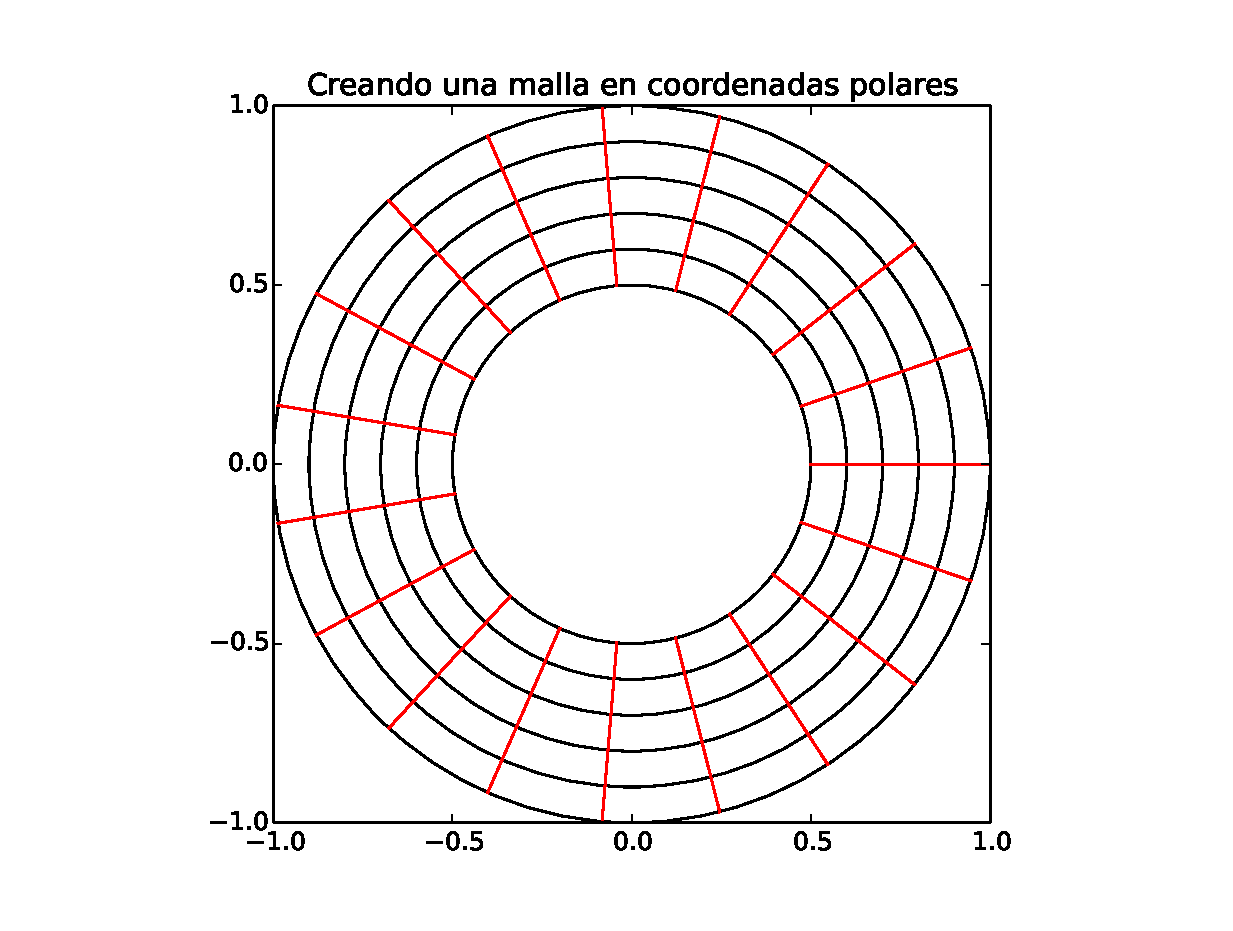
\includegraphics[scale=0.5]{Malla_Circular01.eps} 
%\end{figure}
%\end{frame}
%\begin{frame}
%Usando la malla:
%\begin{eqnarray*}
%r_{i} &=& i \Delta R \\
%\theta &=& j \Delta \theta
%\end{eqnarray*}
%Se aproxima la ecuación por
%\[ \begin{split}
%\dfrac{1}{r_{i}} \left( r_{i+\frac{1}{2}} \dfrac{V_{i+1,j} - V_{ij}}{\Delta r} - r_{j+\frac{1}{2}} \dfrac{V_{ij}-V_{i-1,j}}{\Delta r} \right) \dfrac{1}{\Delta r} + \\
%+ \dfrac{1}{r^{2}} \dfrac{V_{i,j+1}-2V_{ij}+V_{i,j-1}}{\Delta \theta^{2}} = - \dfrac{\rho(r,\theta)}{\epsilon_{0}}P
%\end{split} \]
%\end{frame}
%\begin{frame}
%donde $V_{ij}$ y $r_{ij}$ son funciones
%\[ (r_{i}, \theta_{j}) = (i \Delta r, j \Delta \theta) \]
%Las funciones son periódicas de $j$ en la malla, con período $j=\dfrac{2 \pi}{\Delta \theta}$  y $V_{ij}$ es independiente de $j$.
%\end{frame}
\end{document}
